%\documentclass[iop]{emulateapj-rtx4}
% \shortauthors{French $\&$ Wakker}
%
%\usepackage{graphicx}
%\usepackage{subfigure}
%\usepackage{hyperref}
%\usepackage{amsmath}


%%%%%%%%%%
\documentclass[twocolumn,tighten]{aastex6}
%\documentclass{aastex6}
%\usepackage{emulateapj-rtx4}
%\usepackage{emulateapj}

 \shortauthors{French $\&$ Wakker}
\usepackage{graphicx}
\usepackage{subfigure}


\newcommand{\kms}{$\rm km\, s^{-1}$}
\newcommand{\HI}{H\,{\sc i}}



\graphicspath{{figures//}}

\begin{document}

\title{Do Ly$\alpha$ absorbers co-rotate with galaxy disks?}

\author{David M. French, Bart P. Wakker}

\affil{Department of Astronomy, University of Wisconsin, Madison, WI 53706, USA}

\begin{abstract}

We present results of a study comparing the relative velocity of Ly$\alpha$ absorbers to the rotation direction and velocity of nearby galaxy disks. We find...

\end{abstract}


\keywords{galaxies:intergalactic medium, galaxies:evolution, galaxies:halos, quasars: absorption lines}


\section{INTRODUCTION}
Our current $\Lambda$CDM cosmology picture describes galaxies forming hierarchically out of overdensities in the underlying dark matter distribution. As matter is funneled toward a growing galaxy, conservation of angular momentum redistributes the angular momentum in this gas to match that of the halo and underlying dark matter as the gas is shock-heated and slowly cools. As this infalling gas is responsible for birthing and continuing to feed the galaxies, it is expected that the extended gaseous halos should rotate in the same sense as both the galactic disks and dark matter halos. Galaxy rotation curves have been observed to extend at constant velocity out to... (cite...). It becomes increasingly difficult to measure gas rotation much farther from this however as the density rapidly decreases. Within this region the galaxy disks transition into circumgalactic medium (CGM), and eventually the CGM merges with the intergalactic medium (IGM). At what point, however, does the surrounding medium cease to circulate with the galaxy? 

HYDRO? simulations such as those by \cite{stewart2011, stewart2013} suggests that the bulk CGM kinematics out to (WHAT DISTANCE) may circulate, and that absorption in intervening QSO sightlines should be able to accurately capture this rotation signature. Observational confirmation, however, has be inconclusive. C\^{o}t\'{e} et al. 2005 probed the halos of nine galaxies using \emph{HST} observed background QSOs, finding large warps would be needed to explain the velocity of \HI~absorbers by an extended rotating disk. \cite{wakker2009} compiled a sample of 4 galaxy-QSO systems from the literature, finding only 1/4 of Ly$\alpha$ absorbers appeared to co-rotate with the associated galaxy disk. Approaching the question from a different angle, \cite{bowen2016} probed the halo of a single galaxy, NGC1097, with 4 nearby QSO sightlines, and suggests that an extended, slowly rotating disk with additional inflowing IGM material best matches observations.

%There have been several studies with a sample size of one or a few aiming to compare the kinematics of the galaxy disk to absorption detected in it's CGM halo (e.g., C\^{o}t\'{e} et al. 2005; Wakker \& Savage 2009; Bowen et al. 2016; \textbf{MORE}). With these individual results we may be missing the forest for the sake of the individual trees. There has yet to be a more systematic search for observational evidence that the CGM is kinematically associated with galaxies in general.

Numerous studies have shown a correlation between equivalent width and decreasing velocity difference between galaxies and IGM absorbers (e.g., \citealt{french2017}, MORE).

To make progress here, we have obtained rotation curves for 12 nearby spiral galaxies which are located within 500 kpc of a background QSO observed by the Cosmic Origins Spectrograph (COS) on \textit{HST}. 

We have augmented this new sample with additional galaxies with known rotation velocity and orientation from the literature. In Section 2 we describe the selection and reduction of both SALT and COS spectra. We then discuss each galaxy-QSO system in detail in Section 3, and introduce our halo-velocity model for interpreting these systems in Section 4. In Section 5 we discuss the overall results of this exercise and present a physically-motivated interpretation of these results. See Section 6 for a summary of our results and conclusions.




\begin{table*}[ht]\footnotesize
\begin{center}
\begin{tabular}{l l l l l l l l l l c}
 \hline \hline
  Target 					& Galaxy				& R.A. 				& Dec. 				& \textit{z}		& Program 	 & Cyl. Vel. Range		& NFW Vel. Range	& $T_{exp}*$	   & S/N*  \\ 
  	    					& 	       				&	  				& 		  	 		& 		    	& 		  	 & [\kms]	  	   		& [\kms]	     		& [ks]		   & [1238] \\ 
 \scriptsize (1)  				& \scriptsize (2) 		& \scriptsize (3) 		& \scriptsize (4) 		& \scriptsize (5) & \scriptsize (6) & \scriptsize  (7) 		& \scriptsize (8) 	& \scriptsize (9) & \scriptsize (10)  \\ \hline \hline
\\
%1H0717+714		  							&  	07  21  53.3  		&     +71  20  36.0  		&    0.5003  	& 12025  		&   G130M  			&   LBG812		&  6.0    &      37         \\
1H0419-577  				&      NGC1566  		&      04  26  00.7  		&	-57  12  02.0  		&   0.10400  	& 11686		&   [49, 77]			&   [-2, 31]			& 20429  &      75         \\
%1H0419-577  				&      NGC1566  		&      04  26  00.7  		&	-57  12  02.0  		&   0.10400  	& 11686		&   G160M			&   Obs ID  		& 15934  &      55         \\
HE0429-5343  				&      NGC1566  		&      04  30  40.0  		&	-53  36  56.0 		&   0.04001  	& 12275		&   [-54, -2]			&   [-22, 17]  		& 2067  &       12         \\
HE0435-5304  				&      NGC1566  		&      04  36  50.9  		&      -52  58  47.0  		&   0.42616  	& 11520		&   [-45, -43]			&   [-16, -15]  		& 8372  &       12         \\
%HE0435-5304  			&      NGC1566  		&      04  36  50.9  		&	-52  58  47.0  		&   0.42616  	& 11520		&   G160M			&   Obs ID  		& 8935  &       9           \\
%HE0435-5304  			&      NGC1566  		&      04  36  50.9  		&	-52  58  47.0  		&   0.42616  	& 11520		&   G285M			&   Obs ID  		& 4286  &       2           \\
RBS567  					&      NGC1566  		&      04  39  38.7  		&	-53  11  31.0  		&   0.24300  	& 11520		&   [N/A]				&   [N/A]	  		& 8176  &       17         \\
%RBS567  				&      NGC1566  		&      04  39  38.7  		&	-53  11  31.0  		&   0.24300  	& 11520		&   G160M			&   Obs ID  		& 8933  &       11         \\
%RBS567  				&      NGC1566  		&      04  39  38.7  		&	-53  11  31.0  		&   0.24300  	& 11520		&   G285M			&   Obs ID  		& 4286  &       2           \\
HE0439-5254  				&      NGC1566  		&      04  40  12.0  		&	-52  48  18.0  		&   1.05300  	& 11520		&   [N/A]				&   [N/A]	  		& 8402  &       18         \\
%HE0439-5254			&      NGC1566  		&      04  40  12.0  		&	-52  48  18.0  		&   1.05300  	& 11520		&   G160M			&   Obs ID  		& 8935  &       13         \\
%HE0439-5254 			&      NGC1566  		&      04  40  12.0  		&	-52  48  18.0  		&   1.05300  	& 11520		&   G285M			&   Obs ID  		& 4316  &       2           \\
H1101-232  				&      NGC3513  		&      11  03  37.7  		&	-23  29  31.0  		&   0.18600  	& 12025		&   [-36, 29]			&   [-35, 33]  		& 13341  &      16         \\
%H1101-232  				&      NGC3513  		&      11  03  37.7  		&	-23  29  31.0  		&   0.18600  	& 12025		&   G160M			&   Obs ID  		& 13296  &      10         \\
SDSSJ112005.00+041323.0  	& 	NGC3633  		&      11  20  05.0  		&	+04  13  23.0 		&   0.54689  	& 12603		&   [-155, -12]			&   [-77, 13]  		& 4708  &       9            \\
RX\_J1121.2+0326  			&      CGCG039-137 		&   	11  21  14.0  		&	+03  25  47.0 		&   0.15200  	& 12248		&   [-36, 138]			&   [-36, 166]  		& 2695  &       5           \\
RX\_J1121.2+0326  			&      NGC3633  		&	11  21  14.0  		&	+03  25  47.0 		&   0.15200  	& 12248		&   [-155, -12]			&   [-77, 13]  		& 2695  &       5          \\
%RX\_J1121.2+0326  		&      CGCG039-137 		&	11  21  14.0  		&	+03  25  47.0 		&   0.15200  	& 12248		&   G160M			&   Obs ID  		& 4741  &       4           \\
%RX\_J1121.2+0326  		&      NGC3633  		&      11  21  14.0  		&	+03  25  47.0 		&   0.15200  	& 12248		&   G160M			&   Obs ID  		& 4741  &       4           \\
SDSSJ112224.10+031802.0  	& 	CGCG039-137 		&  	11  22  24.1  		&	+03  18  02.0 		&   0.47528  	& 12603		&   [-130, -114]			&   [-116, -98]  		& 7588  &       10          \\
3C273.0  					&	NGC4536  		&      12  29  06.7  		&	+02  03  09.0 		&   0.15834  	& 12038		&  [67, 134]			&   [-6, 43]  		& 4002  &       111         \\
%3C273.0  				&      NGC4536  		&      12  29  06.7  		&	+02  03  09.0 		&   0.15834  	& 1029		&   G130H				&   Obs ID  		& 10480  &      0            \\
%3C273.0  				&      NGC4536  		&      12  29  06.7  		&	+02  03  09.0 		&   0.15834  	& 1029		&   G190H				&   Obs ID  		& 2880  &       0            \\
%3C273.0  				&      NGC4536  		&      12  29  06.7  		&	+02  03  09.0 		&   0.15834  	& 1029		&   G270H				&   Obs ID  		& 1440  &       0            \\
%3C273.0  				&      NGC4536  		&      12  29  06.7  		&	+02  03  09.0  		&   0.15834  	& 3088		&   G190H				&   Obs ID  		& 5416  &       0            \\
%3C273.0  				&      NGC4536  		&      12  29  06.7  		& 	+02  03  09.0  		&   0.15834  	& 3088		&   G270H				&   Obs ID  		& 5416  &       0            \\
%3C273.0  				&      NGC4536  		&      12  29  06.7  		&	+02  03  09.0 		&   0.15834  	& 1140		&   G160M			&   Obs ID  		& 30028  &      55         \\
%3C273.0  				&      NGC4536  		&      12  29  06.7  		& 	+02  03  09.0  		&   0.15834  	& 1140		&   G200M			&   Obs ID  		& 979  &        10           \\
%3C273.0  				&      NGC4536  		&      12  29  06.7  		&	+02  03  09.0  		&   0.15834  	& 1140		&   G270M			&   Obs ID  		& 1958  &       14          \\
%3C273.0  				&      NGC4536  		&      12  29  06.7  		&	+02  03  09.0  		&   0.15834  	& 8017		&   E140M				&   Obs ID  		& 18671  &      23         \\
HE1228+0131  				&      NGC4536  		&      12  30  50.0  		&	+01  15  23.0  		&   0.11700  	& 11686		&   [23, 131] 			&   [7, 33]  		& 11036  &      61          \\
%HE1228+0131  			&      NGC4536  		&      12  30  50.0  		&	+01  15  23.0  		&   0.11700  	& 11686		&   G160M			&   Obs ID  		& 11029  &      45          \\
%HE1228+0131  			&      NGC4536  		&      12  30  50.0  		&	+01  15  23.0  		&   0.11700  	& 6410		&   G160M			&   Obs ID  		& 11750  &      10           \\
%HE1228+0131  			&      NGC4536  		&      12  30  50.0  		&	+01  15  23.0  		&   0.11700  	& 7737		&   E140M				&   Obs ID  		& 27228  &      9            \\
%LBQS1230-0015  			&      NGC4536  		&      12  33  04.1  		&	-00  31  34.0  		&   0.47095  	& 11598		&   G130M			&   Obs ID  		& 10323  &      13          \\
%LBQS1230-0015  			&      NGC4536  		&      12  33  04.1  		&	-00  31  34.0  		&   0.47095  	& 11598		&   G160M			&   Obs ID  		& 5896  &       7            \\
%PG1302-102  			&      NGC4939  		&      13  05  33.0  		&	-10  33  20.0  		&   0.27840  	& 8306		&   E140M				&   Obs ID  		& 22119  &      7            \\
PG1302-102  				&      NGC4939  		&      13  05  33.0  		&	-10  33  19.0  		&   0.27840  	& 12038		&   [-219, 14]			&   [-119, 36]  		& 5979  &       27          \\
%PG1302-102  			&      NGC4939  		&      13  05  33.0  		&	-10  33  19.0  		&   0.27840  	& 12038		&   G160M			&   Obs ID  		& 6867  &       34          \\
%PG1302-102  			&      NGC4939  		&	13  05  33.0  		&	-10  33  19.0  		&   0.27840  	& 3791		&   G130H				&   Obs ID  		& 18530  &      0            \\
%PG1302-102  			&      NGC4939  		&      13  05  33.0  		&	-10  33  19.0  		&   0.27840  	& 3222		&   G190H				&   Obs ID  		& 2442  &       0           \\
%PG1302-102  			&      NGC4939  		&      13  05  33.0  		&	-10  33  19.0  		&   0.27840  	& 3222		&   G270H				&   Obs ID  		& 939  &        0            \\
SDSSJ135726.27+043541.4  	&	NGC5364  		&      13  57  26.3  		&	+04  35  41.0  		&   1.23453  	& 12264		&   [-38, 123]			&   [-41, 80]  		& 14148  &      15           \\
%SDSSJ135726.27+043541.4	& 	NGC5364  		&      13  57  26.3  		&	+04  35  41.0  		&   1.23453  	& 12264		&   G160M			&   Obs ID  		& 28206  &      12          \\
QSO1500-4140  			&      NGC5786  		&      15  03  34.0  		&	-41  52  23.0  		&   0.33500  	& 11659		&   [120, 175]			&   [26, 69]  		& 9258  &       9           \\
SDSSJ151237.15+012846.0  	& 	UGC09760  		&      15  12  37.2  		&	+01  28  46.0  		&   0.26625  	& 12603		&   [-30, 30]			&   [-30, 95]  		& 7590  &       6           \\
RBS1768  				&      ESO343-G014  	&   	21  38  49.9  		&	-38  28  40.0  		&   0.18299  	& 12936		&   [-203, 10]			&   [-122, 30]  		& 6962  &       24          \\
%RBS1768  				&      ESO343-G014  	&	21  38  49.9  		&	-38  28  40.0  		&   0.18299  	& 12936		&   G160M			&   Obs ID  		& 3837  &       11           \\
MRC2251-178  			&      MCG-03-58-009  	& 	22  54  05.9  		&	-17  34  55.0  		&   0.06609  	& 12029		&   [-52, 166]			&   [-61, 110]  		& 5515  &       42           \\
%MRC2251-178  			&      MCG-03-58-009  	& 	22  54  05.9  		&	-17  34  55.0  		&   0.06609  	& 12029		&   G160M			&   Obs ID  		& 7125  &       30           \\
%MRC2251-178  			&      MCG-03-58-009  	& 	22  54  05.9  		&	-17  34  55.0  		&   0.06609  	& 6484		&   G130H				&   Obs ID  		& 4740  &       0           \\
%MRC2251-178  			&      MCG-03-58-009  	& 	22  54  05.9  		&	-17  34  55.0  		&   0.06609  	& 6484		&   G190H				&   Obs ID  		& 1730  &       0            \\
%MRC2251-178  			&      MCG-03-58-009  	& 	22  54  05.9  		&	-17  34  55.0  		&   0.06609  	& 6484		&   G270H				&   Obs ID  		& 300  &        0            \\
%MRC2251-178  			&      MCG-03-58-009  	& 	22  54  05.9  		&	-17  34  55.0  		&   0.06609  	& 7345		&   G140M			&   Obs ID  		& 10574  &      32           \\
RBS2000  				&      IC5325  			&      23  24  44.7  		&	-40  40  49.0  		&   0.17359  	& 13448		&   [-46, 5]				&   [-24, 17]  		& 5046  &      18           \\
%RBS2000  				&      IC5325  			&	23  24  44.7  		&	-40  40  49.0  		&   0.17359  	& 13448		&   G160M			&   Obs ID  		& 5726  &       12           \\
\hline
\hline \\

RX\_J1017.5+4702			&      NGC3198			&	10 17 31.0		&	+47 02 25.0  		&   0.33544  	& 13314		&   [-154, -21]			&   [-91, 6]  		& 8655  &    12           \\
SDSSJ101622.60+470643.0	&	NGC3198			&	10 16 22.6		&	+47 06 43.0		&   0.82222	& 11598		&   [-155, -17]			&   [-89, 9]	 		& 4906  &	   11		\\

RX\_J1236.0+2641			&	NGC4565			&	12 36 04.0		& 	+26 41 36.0		&   0.20920	& 12248		&   [-1, 250]			&   [-29, 146]		& 4235	&	11	\\

PG0804+761				&	UGC04238		&	08 10 58.7		&	+76 02 43.0		&   0.10200	& 11686		&   [0, 92]				&   [10, 146]		& 5510	&	64	\\

SDSSJ104335.90+115129.0	&	NGC3351			&	10 43 35.9		&	+11 05 29.0		&   0.79400	& 14071		&   [-101, 13]			&   [-70, 20]		& 4736	&	14	\\



MRK771					&	NGC4529			&	12 32 03.6		&	+20 09 30.0		&   0.06301	& 12569		&   [-103, -40]			&   [-105, -35]		& 1868	&	17	\\

MRK876					&	NGC6140			&	16 13 57.2		&	+65 43 11.0		&   0.12900	& 11524		&   [40, 101]			&   [35, 102]		& 12579	&	65	\\

SBS1503+570				&	NGC5907			&	15 04 55.6		&	+56 49 20.0		&   0.35894	& 12276		&   [31, 228]			&   [-24, 101]		&  5163	&	11	\\
SDSSJ152053.59+571122.1	&	NGC5907			&	15 20 53.7		&	+57 11 23.0		&   0.02952	& 13654		&   [-18, 228]			&   [-42, 114]		&  3753	&	2	\\
RBS1503					&	NGC5907			&	15 29 7.5			&	+56 16 07.0		&   0.09900	& 12276		&   [-228, -9]			&   [-96, 33]		&  1964	&	11	\\

SDSSJ112448.30+531818.0	&	UGC06446		&	11 24 48.3			&	+53 18 19.0		&   0.53151	& 14240		&   [-9, 65]				&   [-15, 61]		&  7920	&	9	\\
RX\_J1117.6+5301			&	UGC06446		&	11 17 40.5			&	+53 01 51.0		&   0.15871	& 14240		&   [35, 47]			&   [25, 35]		&  4943	&	11	\\

SBS1116+523				&	UGC06399		&	11 19 47.9			&	+52 05 53.0		&   0.35568	& 14240		&   [-91, -54]$\dagger$	&   [-80, -42]$\dagger$	&  4949	&	14	\\

CSO1208					&	NGC3726			&	11 40 47.9			&	+46 22 05.0		&   0.115		& 14729		&					&				&  3052	&	13	\\
RX_J1142.7+4625			&	NGC3726			&	11 42 41.2			&	+46 24 36.0		&   0.115		& 14772		&   					&				&  2368	&	7	\\

 \\
\hline

\end{tabular}
\end{center}
  \caption{\small{Summary of COS targets in this sample. *Total exposure time and S/N ratio is given for multi-orbit exposures. $\dagger$ Velocity range based on a 2x4 $R_{vir}$ halo. }}
  \label{target_table}
\end{table*}


\section{DATA AND ANALYSIS}

\subsection{SALT Data}
Our sample contains 12 galaxies observed with the Southern African Large Telescope (SALT) Robert Stobie Spectrograph (RSS) in longslit mode. These 12 were selected from a larger pool of 48 submitted targets by the SALT observing queue. These 48 possible targets were chosen for their proximity to background QSOs whose spectra contained promising Ly$\alpha$ lines. Finally, we only included galaxies with $z \leq 0.33$ ($cz \leq 10,000$ \kms), angular sizes less than 6' to enable easy sky subtraction without taking additional exposures, and surface brightnesses sufficient to keep exposure times below $\sim 1300 s$. Table \ref{salt_targets} summarizes these observations. Data was taken for 2 additional galaxies, NGC3640 and NGC2962, but proved unusable due to issues with spectral identification and low signal-to-noise (respectively).

%All SALT galaxy spectra were reduced and extracted using the standard PySALT reduction package (\textbf{\begin{table*}[ht]\footnotesize. 


All SALT galaxy spectra were reduced and extracted using the standard PySALT reduction package (\textbf{CITATION}), which includes procedures to prepare the data, correct for gain, cross-talk, bias, and overscan, and finally mosaic the images from the 3 CCDs. Next, we rectify the images with wavelength solutions found via Ne and Ar arc lamp spectra line identification. Finally, we perform a basic sky subtraction using an off-sky portion of the spectrum, and extract 5-10 pixel wide 1-D strips from the reduced 2-D spectrum. 

For each 1-D spectrum, we identify the H$\alpha$ emission lines and perform a non-linear least-squares Voigt profile fit using the Python package LMFIT\footnote{\url{http://cars9.uchicago.edu/software/python/lmfit/contents.html}}. The line centroid and 1$\sigma$ standard errors are returned, and these fits are then shifted to rest-velocity based on the galaxy systemic redshift and heliocentric velocity corrections are calculated with the IRAF rvcorrect procedure. The final rotation velocity is calculated by then applying the inclination correction, $v_{rot} = v / \sin(i)$. Final errors are calculated as a quadrature sum of $1\sigma$ fit errors, systemic redshift error, and inclination uncertainty as follows:

%\begin{equation}
%\begin{split}
%	\sigma^2 = \left( \frac{\partial v_{rot}}{\partial \lambda_{obs}} \right)^2 (\Delta \lambda_{obs})^2 + \left(\frac{\partial v_{rot}}{\partial v_{sys}} \right)^2 (\Delta v_{sys})^2 + \\
%	\left( \frac{\partial v_{rot}}{\partial i} \right)^2 (\Delta i)^2,
%\end{split}
%\end{equation}

\begin{eqnarray}
	\nonumber
	\sigma^2 = \left( \frac{\partial v_{rot}}{\partial \lambda_{obs}} \right)^2 (\Delta \lambda_{obs})^2 + \\
	\nonumber
	\left(\frac{\partial v_{rot}}{\partial v_{sys}} \right)^2 (\Delta v_{sys})^2 + \\
	\left( \frac{\partial v_{rot}}{\partial i} \right)^2 (\Delta i)^2,
\end{eqnarray}



\noindent where $\Delta \lambda_{obs}$, $\Delta v_{sys}$, and $\Delta i$ are the errors in observed line center, galaxy redshift, and inclination, respectively. 

We determine the inclination error by calculating the standard deviation of the set of all axis ratio values available in NED for each galaxy. The final physical scale is calculated using the SALT image scale of 0.1267 arcsec/pixel, multiplied by the 4-pixel spatial binning, and converted to physical units using a redshift-independent distance if available, and a Hubble flow estimate if not. We adopt a Hubble constant of $H_0$ = 71 \kms $\rm Mpc^{-1}$ throughout.

Finally, we calculate our approaching and receding velocities via a weighted mean of the outer 1/2 of each rotation curve, with errors calculated as weighted standard errors in the mean. Our final redshifts are calculated by forcing symmetric rotation, such that the outer 1/2 average velocity for each side matches in magnitude. See Figure \ref{rotationcurve} for an example.

%\begin{figure}[b!]
%        \centering
%        \vspace{0pt}
%        \includegraphics[width=0.50\textwidth]{NGC3633_2_rotation_curve_xphys_helio_vobs_vrotObs_new4.pdf}
%        \caption{\small{Rotation curve of NGC3633. The solid green line indicates the weighted mean velocity over the corresponding x-axis region, and the shaded green indicates the 1$\sigma$ error in the mean.}}
%        \label{completeness}
%\end{figure}

%\begin{figure}[t!]
%\centering
%  \subfigure[]{\includegraphics[width=1.\linewidth]{NGC3633_2_rotation_curve_xphys_helio_vobs_vrotObs_new4.pdf}}{\label{rotationcurve}}
%  \subfigure[]{\includegraphics[width=0.95\linewidth]{NGC3633_FindingChart.pdf}\label{finderchart}}
%  \caption{\small{a) Rotation curve of NGC3633. The solid green line indicates the weighted mean velocity over the corresponding x-axis region, and the shaded green indicates the 1$\sigma$ error in the mean. b) SALT finder chart for NGC3633 showing the position of the slit in red.}}
%\vspace{5pt}
%\end{figure}



\begin{table*}[ht]\footnotesize. 
\begin{center}
\begin{tabular}{l l l l l l l l l l}
 \hline \hline
%  Galaxy 		 	& R.A. 			& Dec. 		 	& \textit{cz}		& Type		& Grating		& LOS Velocity		& Inc. Corrected Velocity	& Obs Date	& $T_{exp}$		\\ 
  Galaxy 		 	& R.A. 			& Dec. 		 	& \textit{cz}		& Type		& Grating		& $\rm V_{rot}$		& $\rm V_{rot} / \sin(\emph{i})$	& Obs Date	& $T_{exp}$		\\ 

  	    		 	& 	       			&	  		 	& (\kms)			& 		  	&			& [\kms]		     	& [\kms]					&			& [ks]			\\ 
 \scriptsize (1)  	 	& \scriptsize (2)		& \scriptsize (3) 	& \scriptsize (4)		& \scriptsize (5)	& \scriptsize (6)	& \scriptsize (7)		& \scriptsize (8)				& \scriptsize (9)	& \scriptsize (10)	\\ \hline \hline
 
 CGCG039-137 	& 11 21 26.95		& +03 26 41.68		& $6918 \pm24$	& Scd		& PG2300		& $132 \pm 16$	& $139 \pm 26$			& 05 11 2016	& 700			\\ %done
 
 ESO343-G014	 	& 21 37 45.18		& $-$38 29 33.22	& $9139 \pm32$	& S			& PG2300		& $203 \pm 32$	& $203 \pm 32$			& 05 16 2016	& 1000			\\ %done
 
 IC5325		 	& 23 28 43.43		& $-$41 20 0.49	& $1512 \pm8$		& SAB(rs)bc	& PG2300		& $53 \pm 5$		& $125 \pm 39$			& 05 17 2016	& 600			\\ %done
 
 MCG-03-58-009	& 22 53 40.85		& $-$17 28 44.00	& $9015 \pm19$	& Sc			& PG2300		& $150 \pm 12$	& $171 \pm 23$			& 05 16 2016	& 1200			\\ %done

 NGC1566		& 04 20 0.42		& $-$54 56 16.12	& $1502 \pm15$	& SAB(rs)bc	& PG2300		& $64 \pm 8$		& $195 \pm 47$			& 10 18 2016	& 400			\\ %done

 NGC3513		& 11 03 46.08		& $-$23 14 43.8	& $1204 \pm12$	& SB(s)c		& PG2300		& $11 \pm 10$		& $22 \pm 24$				& 05 26 2016	& 600			\\ %done
 
 NGC3633	 	& 11 20 26.22		& +03 35 8.20		& $2587 \pm7$		& SAa		& PG2300		& $149 \pm 6$		& $157 \pm 9$				& 05 11 2016	& 1200			\\ %done

 NGC4536	 	& 12 34 27.05		& +02 11 17.30		& $1867 \pm33$	& SAB(rc)bc	& PG2300		& $129 \pm 9$		& $148 \pm 41$			& 05 11 2016	& 1300			\\ %done

 NGC4939		& 13 04 14.39		& $-$10 20 22.60	& $3093 \pm33$	& SA(s)bc		& PG2300		& $204 \pm 25$	& $275 \pm 66$			& 05 14 2016	& 500			\\ %done

 NGC5364	 	& 13 56 12.00		& +05 00 52.09		& $1238 \pm17$	& SA(rs)bc pec	& PG2300		& $130 \pm 13$	& $155 \pm 22$			& 05 11 2016	& 700			\\ %done
 
 NGC5786	 	& 14 58 56.26		& $-$42 00 48.10	& $2975 \pm22$	& SAB(s)bc	& PG2300		& $156 \pm 10$	& $172 \pm 25$			& 05 11 2016	& 250			\\ %done

 UGC09760	 	& 15 12 02.44		& +01 41 55.46		& $2094 \pm16$	& Sd			& PG2300		& $46 \pm 10$		& $46 \pm 16$				& 05 11 2016	& 500			\\


 \hline

\end{tabular}
\end{center}
  \caption{\small{SALT targeted galaxies. Columns are as follows: 1) the galaxy name, 2), 3) R.A., Dec. in J2000, 4) galaxy systemic velocity, 5) morphological type (RC3), 6) RSS grating used, 7) approaching side velocity, 8) receding side velocity, 9) observation date, 10) exposure time, and 11) S/N of the H$\alpha$ or Ca H\&K lines.}}
  \label{salt_targets}
\end{table*}

\subsection{COS Spectra}
The Barbara A. Mikulski Archive for Space Telescopes (MAST) archives yield 19 QSO targets observed by COS which lie within 500 kpc of our SALT galaxies. These targets vary widely in signal-to-noise from approximately 5 to 100 due to our choosing them based only on their proximity to galaxies with known rotation. The reduction procedure for these spectra follow those described by \cite{french2017} and \cite{wakker2015}. In short, spectra are processed with CALCOS vXXXX? and combined via the method of \cite{wakker2015}, which helps corrects the COS wavelength scale misalignments produced by CALCOS. Multiple exposures are combined via alignment with Galactic 21cm absorption spectra and summing total counts per pixel before converting to flux. The COS instrument is described in detail by \cite{green2012}.


\section{Halo Rotation Model}
In order to better understand how QSO sightlines probe intervening velocity structure we have developed a simple halo gas rotation model. This model is seeded by an observed rotation curve (or whatever rotation curve-esque data suits ones fancy). This input curve is then interpolated and extended out to 2$R_{vir}$ based on the average velocity of the outer 1/2 radius. Next, we project this interpolated rotation curve onto a plane oriented to a faux QSO sightline identically to the input galaxy-QSO pair orientation. By stacking multiple rotation-planes in the galaxy z-axis direction, we then create a simple cylindrical rotating halo model. Finally, each rotation-plane in the stack is projected onto the faux sightline. The result is a function representing the rotation velocity encountered by the sightline as a function of velocity (or distance) along it.

For each galaxy-QSO pair we created 2 rotation models: 1) a purely cylindrical halo extending 2$R_{vir}$ in height and 3$R_{vir}$ in radius, and 2) a cylindrical model extending 2$R_{vir}$ in height and 3$R_{vir}$ in radius with rotation velocities which smoothly decline based on a NFW profile fit \citep{navarro1996, navarro1997}. Each model produces the velocity a co-rotating absorber would project onto the spectrum as a function of velocity along the sightline. We then collapse this into a simple range of possible observed velocities by summing the x- and y-components along the allowed range.

% NFW profile comes from de Blok 2008


\section{SALT Galaxies}

\subsection{CGCG039-137}

CGCG039-137 is an isolated Scd type galaxy with a measured systemic velocity of $6918 \pm 24$ \kms~and inclination of $63^{\circ}$. There are two associated sightlines: RX\_J1121.2+0326 at an impact parameter of 99 kpc and azimuth angle of $71^{\circ}$ on the receding side, and SDSSJ112224.10+031802.0 at 491 kpc and $24^{\circ}$ on the approaching side. Ly$\alpha$ absorption is detected in both sightlines within $400$\kms~ of CGCG039-137. 

Towards RX\_J1121.2+0326 we detect Ly$\alpha$ at 6975 \kms~, which, at $\Delta v = 57$ \kms, lies well within the range of projected velocities consistent with co-rotation. The absorber detected toward SDSSJ112224.10+031802.0 occurs at a more distant 6606 \kms ($\Delta v = -312$ \kms). Although this absorber has the correct sign for co-rotation (blue-ward on the approaching side of the disk), the large velocity difference and impact parameter make it unlikely that this absorption can be linked to coherent halo rotation.


%Systemic velocity as published: 6902
%Velocity as measured: 6917.8 $\pm$ 23.7
%Rotation velocity (inc corrected) 139 $\pm$ 26 \kms
%Rotation velocity (observed) 132 $\pm$ 16 \kms
%Inclination: 61
%Adjusted Inc: 63
%Morphology: Scd
%$L_{\**}$ = 0.62 \\
%
%Two sightlines: \\
%RX\_J1121.2+0326 at 99 kpc, 71deg az: \\
%6975 Lya (dv = 75 \kms on pos side)
%
%SDSSJ112224.10+031802.0 at 491 kpc, 24deg az : \\
%6606 Unmarked (dv = -312 \kms on neg side)


\subsection{ESO343-G014}
ESO343-G014 is an edge on spiral galaxy with a measured systemic velocity of 9138.9 $\pm$ 31.7 \kms. It has a smaller neighboring galaxy, 2MASXJ21372816-3824412, located north of it's major axis at a projected distance of 216 kpc and velocity of 9129. The nearest sightline is towards RBS1768 at an impact parameter of 466kpc and $74^{\circ}$ azimuth angle on the approaching side. We detect 3 Ly$\alpha$ absorption lines within 300 \kms of ESO343-G014 (at 9308, 9360, and 9434 \kms). All of these are anti-aligned with the rotation of ESO343-G014, but unfortunately the presence of 2MASXJ21372816-3824412 makes it difficult to attribute this gas solely to ESO343-G014. Additionally, this gas could be attributed to either the approaching or receding side of the disk due to the large impact parameter and high azimuth angle of the sightline.


%Systemic velocity as published: 9162
%Velocity as measured: 9138.9 $\pm$ 31.7
%Rotation velocity (inc corrected) 205 $\pm$ 53 \kms
%Rotation velocity (observed) 203 $\pm$ 6 \kms
%Inclination: 84
%Adjusted Inc: 90
%Morphology: Sb
%$L_{\**}$ = 1.1 \\
%
%One sightline: \\
%RBS1768 at 466 kpc, 74deg az: \\
%9308 Lya (dv = 169 \kms on pos side)
%9360 Lya (dv = 221 \kms on pos side)
%9434 Lya (dv = 295 \kms on pos side)


\subsection{IC5325}
IC5325 is a face-on SAB(rs)bc type galaxy with a measured velocity of 1511.9 $\pm$ 8.4 \kms. It's inclination is just high enough ($25^{\circ}$) to obtain a reasonable rotation curve. The closest neighboring galaxy is ESO347-G020 to the Southeast at 306 kpc and a heliocentric velocity of 1745 \kms. Three other much smaller galaxies are also located $\sim 450$ kpc to the Southwest. We detect Ly$\alpha$ absorption at 1598\kms, $\Delta v = 86$\kms~in the spectrum towards RBS2000 at an impact parameter of 314 kpc and azimuth angle of $64^{\circ}$ on the approaching side. While this velocity is anti-aligned with the rotation the disk gas, the low inclination angle of IC5325 leads to a highly uncertain position angle. Without additional observations, we cannot say for certain if the location of RBS2000 actually lies on the approaching or receding side. This position angle uncertainty also means our SALT rotation curve is a lower limit on the true rotation velocity of IC5325.

%The velocity of the absorber, $\Delta v = 86$\kms, is also outside the range of projected co-rotation velocities


% Two galaxies are neighboring IC5325 to the South and East: PGC071660 at XXX kpc and NGC7552 at XXX kpc. 
 

%Systemic velocity as published: 1503
%Velocity as measured: 1511.9 $\pm$ 8.4
%Rotation velocity (inc corrected) 125 $\pm$ 45 \kms
%Rotation velocity (observed) 53 $\pm$ 5 \kms
%Inclination: 25
%Adjusted Inc: 25
%Morphology: SAB(rs)bc
%$L_{\**}$ = 0.9 \\
%
%One sightline: \\
%RBS2000 at 314 kpc, 64deg az: \\
%1598 Lya (dv = 86 \kms on possibly? neg side)


\subsection{MCG-03-58-009}
MCG-03-58-009 is a massive and very isolated Sc type galaxy at a measured velocity of $9015 \pm 19$ \kms~ and inclination angle of $49^{\circ}$. A weak Ly$\alpha$ absorber is detected at $9029$ \kms~towards MRC2251-178, which lies 355 kpc away at an azimuth angle of $71^{\circ}$ on the receding side. Although this absorber matches the velocity direction expected for co-rotation, the velocity difference ($\Delta v = 14$ \kms) is within the systemic velocity uncertainty. The relative weakness of this absorber (EW = $62 \pm 4$ m\AA) is somewhat surprising given it's proximity (just outside of 1 $R_{vir}$) to a massive galaxy. If this is representative of an isolated system such as MCG-03-58-009, then we should expect the halo rotational velocity to approach systemic by 1 $R_{vir}$.

%Systemic velocity as published: 9030
%Velocity as measured: 9014.9 $\pm$ 18.6
%Rotation velocity (inc corrected) 171 $\pm$ 24 \kms
%Rotation velocity (observed) 150 $\pm$ 12 \kms
%Inclination: 48
%Adjusted Inc: 49
%Morphology: Sc
%$L_{\**}$ = 2.9 \\
%
%One sightline: \\
%MRC2251-178 at 355 kpc, 71deg az: \\
%9029 Lya (dv = 14 \kms on pos side)



\subsection{NGC1566}
NGC1566 is well sampled (5 nearby QSO sightlines), but unfortunately also part of a complex environment of neighboring galaxies. We detect Ly$\alpha$ in all 5 of these sightlines. The farthest three, HE0439-5254, RBS567, and HE0435-5304, are clustered close together toward the northeast of NGC1566 at 459, 423, and 396 kpc and $\sim 60^{\circ}$ azimuth angle. HE0439-5254 and RBS567 are both located beyond our 2 x 3 $R_{vir}$ model limits and therefore aer only included here for the sake of completeness. The slightly closer HE0435-5304 sneaks under the limit 

HE0429-5343 is in the same direction and azimuth angle but closer at $\rho = 256$ kpc, and shows Ly$\alpha$ absorption at 1167 and 1358 \kms. These absorbers both have the correct velocity \emph{sign}, but we would expect a smaller velocity for co-rotation (approximately $\Delta v \sim \pm40$ \kms~projected). This difference could be explained by invoking either a warped extended disk, or perhaps inflowing gas.

1H0419-577 is located to the south at 303 kpc and just east of the receding side of the major axis at an azimuth angle of $10^{\circ}$. We detect Ly$\alpha$ at 1071, 1123, 1188, 1264, and 2020 \kms, all of which are the wrong sign for co-rotation or distant in velocity. This sightline is actually closer to a small group of galaxies including NGC1549, NGC1546 and NGC1536, all with systemic velocities near $1200$ \kms. We expect the lines at 1071, 1123, 1188, 1264 \kms~to be associated with this group rather than with NGC1566.

%Systemic velocity as published: 1504
%Velocity as measured: 1501.9 $\pm$ 14.9
%Rotation velocity (inc corrected) 86 $\pm$ 21 \kms
%Rotation velocity (observed) 64 $\pm$ 13 \kms
%Inclination: 46
%Adjusted Inc: 48
%Morphology: (R'\_1)SAB(rs)bcSy1
%$L_{\**}$ = 0.59
%Five sightlines: 

% south
%1H0419-577 at 303 kpc, 10deg az: \\
%1071 Lya (dv = -427 \kms on pos side) EW = 249 \pm 2
%1123 Lya (dv = -379 \kms on pos side) EW = 269 \pm 1
%1188 Lya (dv = -314 \kms on pos side) EW = 240 \pm 1
%1264 Lya (dv = -238 \kms on pos side) EW = 91 \pm 2
%2020 Lya (dv = 518 \kms on pos side) EW = 9 \pm 1
%
%% northeast close
%HE0429-5343 at 256 kpc, 60deg az: \\
%1167 Lya (dv = -335 \kms on neg side) EW = 79 \pm 14
%1358 Lya (dv = -144 \kms on neg side) EW = 136 \pm 21
%
%
%% northeast far
%HE0435-5304 at 396 kpc, 62deg az: \\
%1512 Lya (dv = 12 \kms on neg side) EW = 220 \pm 12
%1633 Lya (dv = 131 \kms on neg side) EW = 217 \pm 10
%1690 Lya (dv = 188 \kms on neg side) EW = 204 \pm 11
%
%RBS567 at 423 kpc, 69deg az: \\
%1664 Lya (dv = 162 \kms on neg side) EW = 517 \pm 10
%
%HE0439-5254 at 459 kpc, 65deg az: \\
%1148 Lya (dv = -354 \kms on neg side) EW = 72 \pm 11
%1649 Lya (dv = 147 \kms on neg side) EW = 501 \pm 9



\subsection{NGC3513}
NGC3513 a mostly face-on SB(rs)c galaxy with heliocentric velocity $V_{hel} = 1204 \pm 12$ \kms. It has a companion galaxy in NGC3511 at an impact parameter of 44 kpc at $v_{hel} = 1109$ \kms. We detect Ly$\alpha$ at 1182 \kms~toward background QSO H1101-232, which is located directly south at 60 kpc and azimuth angle of $67^{\circ}$ on the receding side. NGC3513 appears to be rotating slowly, with a maximal inclination-corrected rotation velocity of $22 \pm 24$ \kms. The $\Delta v = -22$ \kms~for this absorber matches well with the magnitude of this rotation, but is opposite in sign for co-rotation. Given that NGC3511 is so close, this absorber's velocity is probably subject to a complex velocity field influenced by both NGC3511 and NGC3513.


%Systemic velocity as published: 1194
%Velocity as measured: 1203.7 $\pm$ 12.0
%Rotation velocity (inc corrected) 20 $\pm$ 22 \kms
%Rotation velocity (observed) 11 $\pm$ 9 \kms
%Inclination: 30
%Adjusted Inc: 30
%Morphology: SB(s)c\_HII
%$L_{\**}$ = 0.49 \\
%
%One sightline: \\
%H1101-232 at 60 kpc, 67deg az: \\
%1182 Lya (dv = -22 \kms on pos side)



\subsection{NGC3633}
NGC3633 is an isolated, edge-on SAa type galaxy at a velocity of $2587 \pm 7$ \kms. Several locations along the disk of NGC3633 show two velocities for emission. We have combined these into a single velocity measurement via a weighted average. 

There are three nearby sightlines: SDSSJ112005.00+041323.0 is straight north at 468 kpc and $78^{\circ}$ azimuth, RX\_J1121.2+0326 is to the southeast at 184 kpc and $58^{\circ}$ azimuth, and SDSSJ112224.10+031802.0 at 413 kpc and $50^{\circ}$ azimuth. Toward RX\_J1121.2+0326 we detect a Ly$\alpha$ absorber at 2605 \kms~on the approaching side, which is essentially systemic velocity for NGC3633. The spectrum of SDSSJ112224.10+031802.0 shows absorbers at 2285 and 2578 \kms, both of which are of the correct sign for co-rotation. We do not detect any Ly$\alpha$ towards the third sightline, SDSSJ112224.10+031802.0.

SDSSJ112005.00+041323.0 and SDSSJ112224.10+031802.0 are both outside of our 2 x 3 $R_{vir}$ model limits.

%We measure a redshift for this galaxy of $cz = 2597.6 \pm 2.4$ \kms. 

%We measure a line-of-sight rotation velocity for NGC3633 of $v_{rot}=139\pm 3.3,~-160\pm5.7$,  \kms.


%Systemic velocity as published: 2600
%Velocity as measured: 2587.2 $\pm$ 6.6
%Rotation velocity (inc corrected) 157 $\pm$ 11 \kms
%Rotation velocity (observed) 149 $\pm$ 6 \kms
%Inclination: 69
%Adjusted Inc: 72
%Morphology: SAa
%$L_{\**}$ = 0.88 \\
%
%Three sightlines: \\
%SDSSJ112005.00+041323.0 at 468 kpc, 78deg az: \\
%2285 Lya (dv = -302 \kms on neg side)
%2578 Lya (dv = -9 \kms on neg side)
%
%
%RX\_J1121.2+0326 at 184 kpc, 58deg az: \\
%2605 Lya (dv = 18 \kms on neg side)
%
%
%SDSSJ112224.10+031802.0 at 413 kpc, 50deg az: \\
%Nothing


\subsection{NGC4536}
NGC4536 is a SAB(rs)bc type galaxy located in a complex environment with many other nearby galaxies. The data on the receding side of NGC4536 is quite messy, and may include contamination from background sources. Hence, our measured systemic velocity of $1867 \pm 33$ \kms, and thus rotation velocity of $139 \pm 37$ \kms, have relatively high uncertainty. Other published redshift values available from NED and rotation velocities from the HyperLEDA database are broadly consistent with our values, albeit biased slightly lower and higher in velocity, respectively.

There are 2 sightlines to the southwest of NGC4536, both on the receding side of the galaxy. HE1228+0131 at 338 kpc and $86^{\circ}$ azimuth has 5 Ly$\alpha$ lines: 1495, 1571, 1686, 1721, and 1854 \kms. None of these are of the correct orientation for co-rotation, and all are more likely to be associated with other nearby galaxies, such as NGC4517A, which is slightly closer to these absorbers in impact parameter and velocity than is NGC4536. The second nearby sightline is toward 3C273 at 344 kpc and $46^{\circ}$ azimuth angle, and shows 3 Ly$\alpha$ lines at velocities of 1580, 2156, 2267 \kms. Two of these are correctly oriented for co-rotation, but are too high in velocity to make this scenario probable. Overall, given the number of nearby galaxies and their locations, we would expect these absorbers to trace the overall velocity field instead of the halo rotation of any particular galaxy.

%However, the approaching side is well sampled and stable with a value of $v_{rot}=-75pm9$ \kms. For this reason, and assuming symmetry for this grand-design spiral galaxy, we have decided to adopt the same value for the receding side, $v_{rot}=75pm9$ \kms.

% The image of this galaxy is confusing - it looks opposite, because we're 'underneath' it (i.e. the near edge is up, the far edge is away). 

%Systemic velocity as published: 1808
%Velocity as measured: 1866.9 $\pm$ 32.9
%Rotation velocity (inc corrected) 139 $\pm$ 37 \kms
%Rotation velocity (observed) 129 $\pm$ 32 \kms
%Inclination: 59
%Adjusted Inc: 61
%Morphology: SAB(rs)bc
%$L_{\**}$ = 2.0 \\

%Three sightlines: \\
%3C273.0 at 344 kpc, 11deg az: \\
%1580 Lya (dv = -287 \kms on pos side)
%2156 Lya (dv = 289 \kms on pos side)
%2267 Lya (dv = 400 \kms on pos side)


%HE1228+0131 at 338 kpc, 76deg az: \\
%1495 Lya (dv = -372 \kms on pos side)
%1571 Lya (dv = -296 \kms on pos side)
%1686 Lya (dv = -181 \kms on pos side)
%1721 Lya (dv = -146 \kms on pos side)
%1854 Lya (dv = -13 \kms on pos side)
%
%2311 Lya (dv = 444 \kms on pos side)

%SDSSJ123748.99+012607.0 at  294 kpc, 37deg az: \\
%not finished


\subsection{NGC4939}
NGC4939 is a large, fast rotating ($V_{rot} = 275 \pm 49$ \kms) SA(s)bc type galaxy at systemic velocity $V_{hel} = 3093 \pm 33$ \kms. We detect a single Ly$\alpha$ absorber at 3448 \kms~towards PG1302-102 at 254 kpc and $61^{\circ}$ azimuth angle towards the southeast. This absorber is located on the approaching side of this galaxy, so we can easily rule out co-rotation in this case. NGC4939 does not have any close neighbors, so represents strong case against co-rotation for gas near or past 1 $R_{vir}$.

%Systemic velocity as published: 3110
%Velocity as measured: 3092.8 $\pm$ 33
%Rotation velocity (inc corrected) 275 $\pm$ 49 \kms
%Rotation velocity (observed) 204 $\pm$ 25 \kms
%Inclination: 46
%Adjusted Inc: 48
%Morphology: SA(s)bc
%$L_{\**}$ = 5.5 \\

%One sightline: \\
%PG1302-102 at 254 kpc, 61deg az: \\
%3448 Lya (dv = 355 \kms on neg side)



\subsection{NGC5364}
NGC5364 is a SA(rs)bc pec type galaxy at a measured systemic velocity of $1238 \pm 17$ \kms. It is located in a group environment with 5 other large, nearby galaxies. The sightline toward SDSSJ135726.27+043541.4 at 165 kpc and $84^{\circ}$ azimuth angle contains Ly$\alpha$ absorbers at 1124 and 1296 \kms~on the receding side. However, because of the orientation of NGC5364 on the sky with respect to this sightline, these absorbers lie extremely close to the inflection point were projected rotation velocities flip to approaching instead of receding. For example, shifting the location of SDSSJ135726.27+043541.4 east by a tenth of a degree ($\sim 20$ kpc) is sufficient to put these absorbers on the approaching side of NGC5364. Hence, both of these absorbers could be co-rotating with NGC5364 given very reasonable assumptions on the shape of an extended disk. Nonetheless, the fact that this system lives in galaxy group environment likely dominates the surrounding velocity field.

%Systemic velocity as published: 1241
%Velocity as measured: 1238.0 $\pm$ 16.9
%Rotation velocity (inc corrected) 155 $\pm$ 27 \kms
%Rotation velocity (observed) 130 $\pm$ 13 \kms
%Inclination: 55
%Adjusted Inc: 57
%Morphology: SA(rs)bc
%$L_{\**}$ = 1.9 \\

%Two sightline: \\
%SDSSJ135309.50+033328.0 at 519 kpc, 21deg az: \\
%not finished
%
%SDSSJ135726.27+043541.4 at 165 kpc, 84deg az: \\
%1124 Lya (dv = -114 \kms on pos? side)
%1296 Lya (dv = 58 \kms on pos? side)


\subsection{NGC5786}
NGC5786 is a large, strongly-barred spiral galaxy at $V_{sys} = 2975 \pm 22$. The sole nearby sightline lies along the major axis on the receding side of NGC5786 at 453 kpc toward QSO1500-4140. Unfortunately for the purpose of this exercise, there are two neighboring galaxies, both of which are closer than this. ESO327-G038 and ESO327-G039 are both located directly south at 62 kpc and 296 kpc, respectively. Toward QSO1500-4140 we detect Ly$\alpha$ absorption at 3138 \kms~, corresponding to a velocity difference $\Delta v = 163$ \kms. Although this velocity aligns nicely with expected co-rotation velocities, the nearby neighboring galaxies and large distance to the absorption ($\sim 2.5 R_{vir}$) make it difficult to believe this as evidence of an extended disk.

%Systemic velocity as published: 2998 \\ 
%Velocity as measured: 2974.6 $\pm$ 21.5 \\
%Rotation velocity (inc corrected) 172 $\pm$ 28 \kms \\
%Rotation velocity (observed) 156 $\pm$ 19 \kms \\
%Inclination: 63 \\
%Adjusted Inc: 65 \\
%Morphology: (R'\_2)SAB(s)bc \\
%$L_{\**}$ = 25 \\
%
%One sightline: \\
%QSO1500-4140 at 453 kpc, 1deg az: \\
%3138 Lya (dv = 166 \kms on pos side) \\


\subsection{UGC09760}
UGC09760 is an edge-on, slow-rotating Sd galaxy with a single sightline toward SDSSJ151237.15+012846.0 located 123 kpc away along the minor axis. Our measured systemic velocity,  $V_{sys} = 2094 \pm 16$, deviates slightly from other published redshifts, such as the The Updated Zwicky Catalog value of $V_{sys} = 2023 \pm 2$ \citep{falco1999}. This is likely due to our method of imposing rotation symmetry and averaging the approaching and receding velocities to derive $V_{sys}$. If we do not sample the rotation curve far enough out, a systematic offset is not unreasonable. Indeed, we do not detect the rotation curve turnover or flattening point.

We detect Ly$\alpha$ absorption at 2051 \kms ($\Delta v = -43$ \kms). This velocity matches well with the rotation velocity of UGC09760 ($V_{rot} = 46 \pm 16$ \kms), but unfortunately this sightlines lies almost exactly at an azimuth of $90^{\circ}$. Hence, the motion of this gas gas could easily be either co-rotating or counter-rotating depending on a minute change in the position angle assigned to UGC09760. This is especially true if we assume our measured $V_{sys}$ is erroneously high, and indeed closer to the values obtained by other observations.

It is worth noting that there are several small satellite galaxies nearby, including SDSSJ151208.16+013508.5, SDSSJ151121.63+013637.6, SDSSJ151241.38+013723.7 and UGC09746 (impact parameters of 53, 88, 82, 230 kpc respectively). All of these galaxies lie slightly blue-ward of UGC09760, and thus \emph{farther} away in velocity from the Ly$\alpha$ absorber at 2051 \kms.

%Systemic velocity as published: 2023 \\
%Velocity as measured: 2093.7 $\pm$ 15.5 \\ 
%Rotation velocity (inc corrected) 46 $\pm$ 16 \kms \\ 
%Rotation velocity (observed) 46 $\pm$ 12 \kms \\ 
%Inclination: 85 \\ 
%Adjusted Inc: 90 \\ 
%Morphology: Sd \\ 
%$L_{\**}$ = 0.17 \\

%Two sightlines:
%SDSSJ151237.15+012846.0 at 123 kpc, 90deg az: \\
%2051 Lya (dv = -43 \kms on minor axis. Looks neg side, but extremely close) \\



\section{Ancillary Data}
To increase our sample size we have also searched the literature for galaxies with published rotation curves and orientations. Unfortunately, while the rotation velocity is available for thousands of galaxies, only a handful also include the \emph{orientation} of the rotation on the sky. Of these, we were able to find 18 additional galaxies which have a systemic velocity greater than $\sim 500$ \kms, and are near to a COS or STIS sightline with available data.

%THINGS:

%\subsection{NGC0628}
%From the THINGS survey \citep{walter2008}, NGC0628 fits our criteria with a heliocentric velocity of 657 \kms~ and a sightline towards SDSSJ014143.20+134032.0 located at 377 projected kpc away. Although NGC0628 is mostly face-on ($i = 31^{\circ}$), we were able to extract a rotation curve from the publicly available THINGS first-moment \HI map.

%Heliocentric velocity = 657kms
%SDSSJ014143.20+134032.0 at 377kpc (absorption at 637, 789) - much closer to another, larger galaxy


\subsection{NGC3198}
NGC3198 is a well studied SB(rs)c type galaxy which is included the detailed THINGS rotation curve study of \cite{deblok2008}. We extracted the raw rotation curve derived by \cite{deblok2008} using the plot digitization software WebPlotDigitizer\footnote{WebPlotDigitizer; http://arohatgi.info/WebPlotDigitizer}. NGC3198 has a systemic velocity of 660 \kms, and is located 370 kpc away from a sightline toward RX\_1017.5+4702 at an azimuth angle of $55^{\circ}$ on the approaching side of NGC3198 (northeast). NGC3198 has an even and flat rotation curve, with an average velocity of $v_{rot} = 152$ \kms and an expected velocity range of [-82, -23] based on our projected NFW profile fit. We detect Ly$\alpha$ absorption in the spectrum of RX\_1017.5+4702 at 629 \kms ($\Delta v = -31$ \kms). Hence, the velocity of this absorber can nicely be described by a co-rotating disk.

SDSSJ101622.60+470643.0 is also located in the same direction but at a more distant 401 kpc away (\textbf{NOT IDENTIFIED}).

The small dwarf galaxy SDSSJ101848.77+452137.0 is located 65 kpc away toward the southwest.

% SDSSJ101950.83+453208.0, SDSSJ101958.45+453341.6, SDSSJ101946.39+453104.7 are PofG in the table


% (see e.g., \cite{begeman1989})
%Heliocentric velocity = 660kms - Begeman 1987, THINGS de Blok paper
%SDSSJ102152.30+464515.0 at 300kpc low res only
%RX_J1017.5+4702 at 370kpc, 55.3 azimuth (line at 629kms) = good
%SDSSJ102839.10+450009.0 at 390kpc (low res only)
%SDSSJ101622.60+470643.0 at 401kpc, 61 azimuth (no IDs, possible line) = pretty far away



\subsection{NGC3351}
At $V_{sys} = 778$ \kms NGC3351 is a mostly face-on ($i = 29^{\circ}$) SB(r)b type galaxy located $\sim200$ kpc southwewst of the core of the Leo I group.  We take the rotation curve and orientation produced by \cite{dicaire2008}. While we expect any extended disk rotation to be quickly disrupted due to the complex Leo I environment, this galaxy also has the closest sightline of our sample with SDSSJ104335.90+115129.0 at 31 kpc and $13^{\circ}$ azimuth on the northwest, approaching side. We detect Ly$\alpha$ at 717, 882, and 1030 \kms ($\Delta v = -61, 104, 252$ \kms) toward this sightline. The lowest velocity absorber agrees nicely with both models for co-rotation, while the other two are too high in velocity. \\

%IRAS10378+1109 - no data (clobbered by LLS) \\
%3C245.0 - low res only \\
%SDSSJ105125.80+124746.0 at 371, 76 az (proprietary until 2019) \\


SDSSJ104335.90+115129.0 at 31kpc, 13 az (Lya at 717, 882, 1030) \\

SDSSJ104816.30+120735.0 at 198kpc, 85 az (G130M but not in reduce) \\
SDSSJ104709.80+130454.0 at 277kpc, 47 az (G130M but not in reduce) \\
SDSSJ104843.50+130605.0 at 317kpc, 57 az (G130M but not in reduce) \\
SDSSJ105220.60+101751.0 at 435kcp, 39 az (not ID'd, possible line) \\ 
SDSSJ104341.53+085558.2 at 484kpc, 18 az (G130M but not in reduce) \\


% see mazzalay2014 also




\subsection{NGC5907}
NGC5907 is a large, edge-on SA(s)c type galaxy at $V_{sys} = 667$ \kms. We have taken the rotation curve and orientation information from \cite{yim2014}. The closest sightline resides toward SDSSJ152053.59+571122.1 on the northwest (receding) side, at 286 kpc and $63^{\circ}$ azimuth. 

%Sanders 1996, Allaert (2015A\&A...582A..18A) also \\
%
%NW is receding side \citep{allaert2015}. \\
%Rotation curve data from \cite{yim2014} \\
 
SDSSJ152053.59+571122.1 at 286 kpc, 63 az (possible line around 880 \kms, messy spectrum, not ID'd) \\
SBS1503+570 at 413 kpc, 47 az (Lya at 708kms) \\
RBS1503 at 478 kpc, 63 az (no lines)




\subsection{NGC4565}
NGC4565 is an edge-on ($i = 75^{\circ}$ SA(s)b type galaxy at a heliocentric velocity of 1230 \kms, for which we have taken the rotation curve and orientation from \cite{sofue1996}. The sightline toward RX\_J1236.0+2641, at 147 kpc and $41^{\circ}$ azimuth angle on receding side, contains Ly$\alpha$ absorbers at velocities of 1009 and 1166 \kms ($\Delta v = -221, -64$ \kms). Both are consistent with counter-rotating gas, although the line at 1166 \kms is close to the allowed range of [-29, 146] for co-rotation. However, the presence of several satellite galaxies surely disrupts any possible extended disk rotation that would otherwise be detectable via sightline absorption.



\subsection{UGC06446}
UGC06446 is an Sd galaxy located at $V_{sys} = 645$ \kms~on the far northwest edge of the Ursa Major cluster of galaxies. We take the rotation curve and orientation information from \citep{verheijen2001, swaters2009}. We detect Ly$\alpha$ absorption toward two nearby QSO's, SDSSJ112448.30+531818.0 at 143 kpc and $22^{\circ}$ azimuth and RX\_J1117.6+5301 at 417 kpc and $52^{\circ}$ azimuth, are both located toward the southwest, receding side of UGC06446. The absorbers residing at 664 \kms~and 685 \kms, respectively, both agree well with the expected velocities for co-rotating gas ([-15, 61], [25, 35]). Interestingly, we note that the more distant absorber toward RX\_J1117.6+5301 has a larger $\Delta v$ value ($\Delta v = 40$ \kms compared to $19$ \kms). If both absorbers were strictly following the expected NFW rotation curve, we would expect the opposite, with the more distant absorber velocity approaching $V_{sys}$.


%SDSSJ112448.30+531818.0 at 143kpc, 22 az (Lya at 664kms) \\
%RX\_J1117.6+5301 at 417kpc, 52 az (Lya at 685kms) \\

%MCG9-19-073 at 179kpc - low res only \\ 
%RBS971 at 226kpc, 88 az (clobbered by huge H2 system) \\

%Check these:
%FBSJ0908 - 200kpc
%1116+523 - 400kpc


\subsection{UGC06399}
UGC06399 is an edge-on Sm type galaxy located at $V_{sys} = 791$ \kms~on the far west edge of the Ursa Major cluster of galaxies. Again, we take the rotation curve and orientation information from \citep{verheijen2001, swaters2009}. As noted by \cite{verheijen2001}, this is the most isolated galaxy in the Ursa Major cluster. Unfortunately, the closest QSO is SBS1116+523, at 471 kpc away on the northwest, approaching side. Although we detect Ly$\alpha$ absorption at 731 \kms, this impact parameter is beyond our model radius of $3 R_{vir}$. Nonetheless, the velocity of this absorber agrees well with the expected velocity range if we extend a static or NFW rotating disk out to $4 R_{vir}$.

%SBS1116+523 at 471kpc, 13.4 az (Lya at 731kms) \\

%MCG9-19-078 at 301kpc (G160M only) \\
% southeast side is receding


\subsection{NGC3726}
 $V_{sys}= 866$ \kms. S side is receding.  \cite{verheijen2001} \\
 

Inclination: 52 \\
Adjusted Inc: 54 \\
Morphology: SAB(r)c \\
$L_{\**}$ = 1.5 \\

CSO1208 at 369kpc, 87 az (Lya at 731, 874kms) \\
RX\_J1142.7+4625 (PGC139665) at 440, 86 az (G130M but not in reduce) close to CSO1208 \\

Both sightlines closer to some other little galaxies. NGC3877 nearby, has rot curve \\



\subsection{NGC3067}
The galaxy-QSO pair NGC3067-3C232 is a particularly well studied system. They are separated by only 11 kpc ($74^{\circ}$ azimuth angle) and a LLS of $N_{HI} = 1 � 10^{20}$ $\rm cm^{-2}$ is detected toward 3C232 at 1421 \kms ($V_{sys} = 1476$ \kms), which has been postulated as a high velocity cloud (HVC) orbiting NGC3067. We obtained the rotation curve for NGC3067 from \cite{danziger1972} and the orientation from \cite{carilli1989} (see also \cite{keeney2005}). \\

Inclination: 68 \\
Adjusted Inc: 71 \\
Morphology: SAB(s)ab \\
$L_{\**}$ = 0.5 \\

SDSSJ095914.80+320357.0 at 128 kpc, 43 az (no ID'd, but probable line around 1500kms) \\
RX\_J1002.9+3240 at 359 kpc, 33 az (not in reduce yet) \\


%%%%%%%%%%%%%%%%%%%%%%%%%%%%%%%%%%%%%%%%
%%%%%%%%%%%%%%%%%%%%%%%%%%%%%%%%%%%%%%%%


We have also included the 5 galaxy-QSO systems analyzed by \cite{cote2005}. We briefly summarize each of these systems here, and refer the reader to \cite{cote2005} for a more complete discussion. \textbf{ALL? OF THESE GALAXIES WE PROJECT TO BE AT GREATER IMPACT PARAMETER THAN COTE DID. MOSTLY BASED ON BETTER RID DISTANCES THAN USED BY COTE}

\subsection{NGC6140}
NGC6140 is a small SB(s)cd\_pec type galaxy located at $V_{sys} = 910$ \kms~and 113 kpc from the sightline toward QSO MRK876. The approaching side is oriented toward the east, with MRK876 toward the northwest at an azimuth of $21^{\circ}$ (although this is somewhat uncertain; the position angle for NGC6140 could be closer to $60^{\circ}$ than our adopted value of $94^{\circ}$ due to it being mostly face on, faint, and strongly barred). We detect Ly$\alpha$ absorption toward MRK876 at 939 \kms ($\Delta v = 29$ \kms). This value implies co-rotation, but is just below the range predicted by our models (35 - 102 \kms).


%Inclination: 44 \\
%Adjusted Inc: 45 \\
%Morphology: SB(s)cd \\
%$L_{\**}$ = 0.2 \\

% HS1626+6433 is low res only and KAZ49 is too far away


\subsection{NGC4529}
As an inclined, isolated galaxy with a QSO sightline located 159 kpc and only $23^{\circ}$ off the major axis, NGC4529 represents an ideal test environment for this study. This sightline towards MRK771 contains a Ly$\alpha$ absorber at 2553 \kms. With $V_{sys} = 2536$ \kms~and MRK771 located on the approaching side of NGC4529 (southwest side), this is a clearcut case of counter-rotating \HI. As \cite{cote2005} conclude, ``there is simply no physical way to produce such a velocity with an extending co-rotating disk." \\

%Inclination: 69 \\
%Adjusted Inc: 72 \\
%Morphology: Scd \\
%$L_{\**}$ = 1.2 \\

% called this in cote 2005:
%UGC07697 - 2535kms -  new COS data
%MRK771 at 159kpc, 23 az (Lya at 2553)


\subsection{UGC04238}
UGC04238 is an isolated and edge-on SBd type galaxy at $V_{sys} = 1544$ \kms. We take the rotation curve and orientation from \cite{cote2005}. Ly$\alpha$ are detected at 1143, 1526, and 1593 \kms toward PG0804+761, located directly south at 148 kpc and $59^{\circ}$ azimuth on the receding side of UGC04238. Only the absorber at 1593 \kms, the lowest $W$ of the three, falls within the expected velocity range for co-rotation. 

% Approaching side to the northeast. \\

%Inclination: 77 \\
%Adjusted Inc: 75 \\
%Morphology: SBd \\
%$L_{\**}$ = 0.58 \\



The following are from \cite{rhee1996}: \\

\subsection{NGC2770}
$V_{sys} = 1947$ \kms. Nearby to small dwarfs MCG+06-20-036NED02 and GALEXASCJ090946.88+330840.4 (both 25 kpc, on opposite sides of NGC2770). \cite{rhee1996} \\

Inclination: 75 \\ 
Adjusted Inc: 80 \\ 
Morphology: SA(s)c \\ 
$L_{\**}$ = 1.8 \\

FBQSJ0908+3246 at 204 kpc, 59 az (Lya at 1915, 1982) \\ 
TON1009 at 267 kpc - used to be identified, but not anymore? \\
TON1015 at 218 kpc, 61 az (Lya at 1833, 1985) \\ 
SDSSJ091052.80+333008.0 at 239 kpc, 66 az (Lya at 1824, 1975) \\
SDSSJ091127.30+325337.0 at 234 kpc, 30 az (Lya at 2063) \\


\subsection{NGC3432}
$V_{sys} = 616$ \kms. Interacting with the nearby dwarf galaxy UGC05983 located 11 kpc away and at $V_{sys} = 765$ \kms. \cite{rhee1996}. \\

Inclination: 78 \\ 
Adjusted Inc: 90 \\ 
Morphology: SB(s)m \\ 
$L_{\**}$ = 0.42 \\

CSO295 at 20 kpc, 82 az (Lya 600, 662) \\ 
RX\_J1054.2+3511 at 290 kpc, 57 az (Looks like a feature around 600 \kms~but no ID?) \\
MS1047.3+3518 at 326 kpc, 26 az (low SN, not ID'd, possible feature?) \\

% note the following entries in the galaxy table are all actually "Part of NGC3432" or PofG - "Part of Galaxy" from NED
% SDSSJ105231.02+363709.6
% SDSSJ105229.19+363649.8
% SDSSJ105233.13+363736.7
% SDSSJ105240.79+363953.7


\subsection{NGC3666}
$V_{sys}=1060$ \kms. Mostly isolated, with only a few dwarfs $\sim400$ kpc away. \cite{rhee1996} \\

Inclination: 73 \\ 
Adjusted Inc: 77 \\ 
Morphology: SA(rs)c \\ 
$L_{\**}$ = 0.61 \\

SDSSJ112439.50+113117.0 at 58 kpc - Borthakur target (not in reduce yet) \\
SDSSJ112632.90+120437.0 at 279 kpc - Borthakur target (not in reduce yet) \\ 
SDSSJ112756.70+115427.0 at 320 kpc - (not in reduce yet) \\
SDSSJ111916.20+110107.0 at 406 kpc - G230L only \\
4C12.40 at 451 kpc - G190H, G270H, G230L only \\

%\subsection{NGC3769}
%$V_{sys} = 737$ \kms. \cite{rhee1996}
%CSO1208 at 459 kpc
% RXJ1142.7+4625 at 485 kpc
% both sightlines are very far away and closer to other stuff. ignore

%\subsection{NGC3949}
%\cite{rhee1996}
%
%SDSSJ115412.10+463552.0 at 402 kpc - closer to something else. Don't bother

%\subsection{NGC4157}
%\cite{rhee1996}
%SBS1215+497 at 440 kpc - (G140L only)
%HS1216+5032B at 379 kpc - (G270H only)
%HS1216+5032A at 379 kpc - (G270H only)
% don't bother

%\subsection{NGC4414}
%$V_{sys} = 716$ \kms. \cite{rhee1996}
%TON618 at 155 kpc (G270H only)
%PG1218+304 at 478 kpc (no lines)

%\subsection{NGC4534}
%\cite{rhee1996}
%KUG1240+359 at 486 kpc
%Don't bother

\subsection{NGC5951}
$V_{sys} = 1780$ \kms. A couple of nearby galaxies (NGC5954, NGC5953), but the sightline is closer and on the opposite side. \cite{rhee1996} \\

Inclination: 78 \\
Adjusted Inc: 86 \\
Morphology: SBc \\
$L_{\**}$ = 1.4 \\

2E1530+1511 at 55 kpc, 85 az  - (Lya at 1795, 1953) \\


%\subsection{NGC7741}
%$V_{sys} = 750$ \kms. Both UGC12732 and UGC12791 are closer than the sightlines. \cite{rhee1996} \\
%
%Inclination: 64 \\
%Adjusted Inc: 66 \\
%Morphology: SB(s)cd \\
%$L_{\**}$ = 0.59 \\
%
%RBS2055 at 388 kpc, 88 az - (no lines) \\
%
%Probably don't bother with non-detections? \\


\subsection{NGC7817}
$V_{sys} = 2309$ \kms. Sightline toward MRK335 is equidistant but opposite NGC7798. \cite{rhee1996} \\

Inclination: 75 \\
Adjusted Inc: 80 \\
Morphology: SAbc \\
$L_{\**}$ = 0.79 \\

MRK335 at 343 kpc, 90 az (Lya at 1954, 2274) \\


\subsection{UGC08146}
$V_{sys} = 670$ \kms. Small but isolated. \cite{rhee1996}. This galaxy also is included in the \cite{cote2005} sample. \\

Inclination: 78 \\
Adjusted Inc: 90 \\
Morphology: Scd \\
$L_{\**}$ = 0.31 \\

PG1259+593 at 114 kpc, 50 az (Lya at 646, 683) \\
SBS1304+594 at 235 kpc, 15 az (no lines, low SN) \\


%\subsection{UGC05459}
%$V_{sys} = 1112$ \kms. \cite{rhee1996}
%SDSSJ100514.20+530240.0 at 157 kpc (G140L only)
%SBS1010+535 at 292 kpc (G140L only)
% no targets


%NGC4579 -  low res only
%NGC4569 - too close
%NGC4501 - no targets
%NGC2683 - too close
%IC0342 - too close
%NGC0253 - too close
%NGC0891 - too close
%NGC1808 - no targets
%UGC02885 - no targets
%NGC4389 - target no good
%NGC3718 - targets closer to other shit
%NGC3893 - cluster
%NGC3877 - cluster
%UGC06667 - no targets
%NGC3769 - no targets
%NGC6674 - no targets
%NGC6503 - too close
%NGC6195 - no targets
%NGC5585 - too close
%UGC09211 - too close

%NGC5533 - no target

%NGC5033 - complicated environment
%CSO952 - low res only

%NGC4455 (Verheijen 2001)
%PG1222+216 at 248kpc (no Lya)
%PG1222+228 at 116kpc (low res only)

%NGC4218 - cluster
%NGC4138 - no targets
%NGC4100 - no targets
%UGC07089 - cluster
%UGC06983 - no targets
%UGC06923 - no targets
%NGC3985 - part of cluster
%UGC06917 - low res only
%NGC3972 - part of cluster
%NGC3953 - no targets
%NGC3949 - too far from target
%NGC3917 - no target
%NGC1365 - low res only
%UGC03137 - no targets
%NGC3274 - no targets
%NGC3109 - too close
%UGC05272 - too close, targets too far
%NGC2998 - no targets
%UGC03371 - no targets
%UGC02885 - no targets
%UGC02849 - no targets
%NGC1324 - no targets
%NGC0801 - no targets
%NGC0247- too close
%NGC0055 - too close

%NGC2903 = 550kms - too close
%SDSSJ093602.10+200543.0 at 255kpc (not in reduce), PG0923+201 at 355kpc (no lines)

%NGC3621
%Heliocentric velocity = 730kms
%PKS1101-325 at 364kpc, 70 az (no lines)

%NGC2841 = 638kms - MRK110 at 357kpc (no lines)

%NGC3079 - Sofue & Rubin 2001, Sofue et al. 2000, Irwin and Seaquist 1991
%QSO0957+5608 at 73 kpc - low res only (also called Q0957+561A)
%SBS0955+560 at 156 kpc - G160M only
%QSO0958+5625 at 156kpc - low res only
%4C55.17 at 213kpc - low res only
%MRK132 at 241kpc - low res only
%SBS0953+549 at 379kpc - low res only


%NGC6691 - no close targets
%IC1132 - no targets
%UGC09837 - no targets
%UGC09177 - no targets
%IC0853 - no targets
%NGC4977 - no targets
%NGC4662 - no targets
%UGC07416 - no targets
%NGC4195 - no targets

%NGC3982	- Martinsson et al 2016
%Part of a group that's closer than the sightline - no good
%PG1148+549 at 337kpc (not fully ID'd, possible line)
%RBS1047 - low res only

%NGC4527 - right in the middle of a complex group
%UGC06903 - low res only
%NGC3949 - sightline >400kpc away
%NGC3687 - no targets
%NGC2649 - no targets
%NGC2599 - no targets
%UGC04380 - no targets
%NGC2575 - no targets
%NGC2532 - no targets
%UGC04107 - no targets
%NGC2441 - no targets
%UGC03997 - no targets
%UGC03701 - no targets
%NGC1642 - no targets
%IC0208 - no targets
%UGC01087 -  no targets
%NGC0234 - no targets
%IC0043 - no targets
%NGC5529 - no targets
%NGC4217 - no targets
%IC2531 - no targets
%UGC04277 - low res only
%NGC0973 - no targets

%NGC4157
%SBS1215+497 - low res only
%HS1216+5032B - low res only
%HS1216+5032A - low res only

%UGC04277 - only a low res target
%UGC02259 - targets too far, too small
%NGC6674 - no targets
%UGC02885 - no targets

%NGC0100 - 841kms
%No lines

%NGC4414 - 716kms - de Blok 2014
%TON618 at 155kpc (low res only)
%PG1218+304 at 478kpc (too far, closer to another galaxy)

%UGC08333 - 935kms - Begeman 1989
%Not ideal as R_vir is 80kpc - closest QSO is >3Rvir
%SDSSJ131447.10+260623.0 at 274kpc, 47az (not in reduce)
%SDSSJ131802.10+262830.0 at 438kpc (Lya at 442 - too far)

%IC2574 - 57kms - too close
%NGC5533 - no targets

%NGC2403 - 133kms - too close - Begeman 1987
%NGC6503 - 25kms - too close - Begeman 1987

%NGC2903 - Too close
%550 kms
%SDSSJ093602.10+200543.0 at 255kpc (not public until November)
%PG0923+201 at 331kpc (too close, no flux here)


%'DDO 23'
%MCG-02-07-026 = 2102kms - QSO0226-1024 at 322.238 kpc, only FOS data?

%'DDO 154'
%NGC4789A = 374kms - too close
%US143 at 125kpc (not reduced), US136 at 136kpc (not reduced), CSO176 at 148.514kpc

%NGC0925 = 553kms - 3C68.1 at 210kpc (G230L only)

%NGC2976 = 3kms - too close

%M81
%NGC3031 = MESSIER081 = too close

%NGC3077 = 14kms - too close
%NGC3184 = 592kms - KUV10128+4055 (G140L only), others similiar

%NGC3521
%Heliocentric velocity = 801kms
%SDSSJ110736.67+000329.4 at 90kpc (low res only)
%PG1103-006 at 169kpc (STIS1200 only, not enough resolution)
%SDSSJ110729.03+004811.1 at 183kpc (low res only)
%SDSSJ110636.79-011454.7 at 240kpc (low res only)
%SDSSJ110936.35+005111.3 at 254kpc (low res only)
%SDSSJ111054.92+004854.2 at 300kpc (low res only)
%SDSSJ111256.13+001343.5 at 352kpc (low res only)


%NGC3627 - super complex environment
%Heliocentric velocity = 727kms
%4C12.40 at 80kpc (low res only)
%SDSSJ112632.90+120437.0 at 291kpc, 66 az (G130M but not in reduce)
%SDSSJ112439.50+113117.0 at 297kpc, 43 az (G130M but not in reduce)
%SDSSJ111916.20+110107.0 at 324kpc (low res only)
%SDSSJ112756.70+115427.0 at 353, 67 az (G130M but not in reduce)
%SDSSJ113210.50+133509.0 at 483kpc, 71 az (G130M but not in reduce)

%NGC4214  = 291kms - too close
%NGC4449 = 207kms - too close
%NGC4736 = 308kms - too close
%
%NGC4826 = 408kms - too close
%RXS_J1251.7+2404	at 246kpc (low res only)
%SDSSJ125846.70+242739.0 at 261 (no lines)
%more...
%
%NGC5055 = 484kms - too close
%KISSR1567 at 355kpc (spectrum no good)
%SDSSJ130631.60+435100.0 at 344kpc (low res only)
%more...
%
%NGC5194 - 463kms - too close
%SDSSJ132909.20+480109.0 at 114kpc (low res only)
%QSO1320+4755 at 175kpc (low res only)
%PB161 at 179kpc (low res only)
%SDSSJ132222.70+464535.0 at 185kpc (G130M, not in reduce)
%more...
%
%NGC5236 - 513kms - too close
%NGC5135 at 207kpc (low res only)
%PKS1349-265 at 383 (low res only)
%more...
%
%NGC5457 - 241kms - too close
%NGC6946 - 40kms - too close
%NGC7331 - 816kms - no targets
%NGC7793 - 230kms - too close



%2) a spherical halo extending 2$R_{vir}$ in radius, and 3) a cylindrical model extending 1$R_{vir}$ in height and 2$R_{vir}$ in radius with rotation velocities which smoothly decline to systemic towards these boundaries.



%\begin{figure}[ht!]
%        \centering
%        \vspace{0pt}
%        \includegraphics[width=0.50\textwidth]{fig1.pdf}
%        \caption{\small{Distribution of $L/L_{\**}$ values for all galaxies in the dataset. Black vertical lines highlight 1, 0.5, 0.1, 0.05 and 0.01 $L_{\**}$. The turnoff around 0.1$L_{\**}$ shows that on average, the dataset is mostly complete to 0.2$L_{\**}$.}}
%%        \vspace{-5pt}
%        \label{completeness}
%\end{figure} 


%\begin{table*}[ht]\footnotesize
%\begin{center}
%\begin{tabular}{l l l l l l l l l l l l l l l}
% \hline \hline
%  $Target$	&  $Galaxy$  & $R_{vir}$        & $v_{galaxy}$ 	   	  &  $Inc.$               &  $Az.$ 	       & $\rho$		   & $v_{Ly\alpha}$	 	  	& $W_{Ly\alpha}$  & $\Delta v$  			 & $\mathcal{L}$ \\ 
%  	  	&       & \scriptsize (kpc) & \scriptsize  $\rm (km ~s^{-1})$ & \scriptsize (deg) & \scriptsize [deg] & \scriptsize (kpc) & \scriptsize  $\rm (km\, s^{-1})$ & \scriptsize $\rm (km\, s^{-1})$ & \scriptsize  $\rm (km\, s^{-1})$ &  \\
% \scriptsize (1) & \scriptsize (2) & \scriptsize (3)    & \scriptsize (4)     & \scriptsize (5)    & \scriptsize (6)   & \scriptsize  (7)   & \scriptsize (8) & \scriptsize (9) & \scriptsize (10) & \scriptsize (11) \\ \hline \hline
%
%1H0717+714  &  UGC03804  &  173  &  2887  &  55  &  7  &  207  &  2870  &  343$\pm$6  &  17  &  0.24  \\
%
%
% \\
%\hline
%\end{tabular}
%\end{center}
%  \caption{\small{All associated systems. The largest $\mathcal{L}$ value is given, with a (\**) indicating that this corresponds to $\mathcal{L}_{d^{1.5}}$, otherwise the quoted $\mathcal{L}$ was computed with $R_{vir}$.}}
%  \label{target_table}
%\end{table*}


\section{Discussion}


\begin{figure*}[ht!]
        \centering
        \vspace{0pt}
        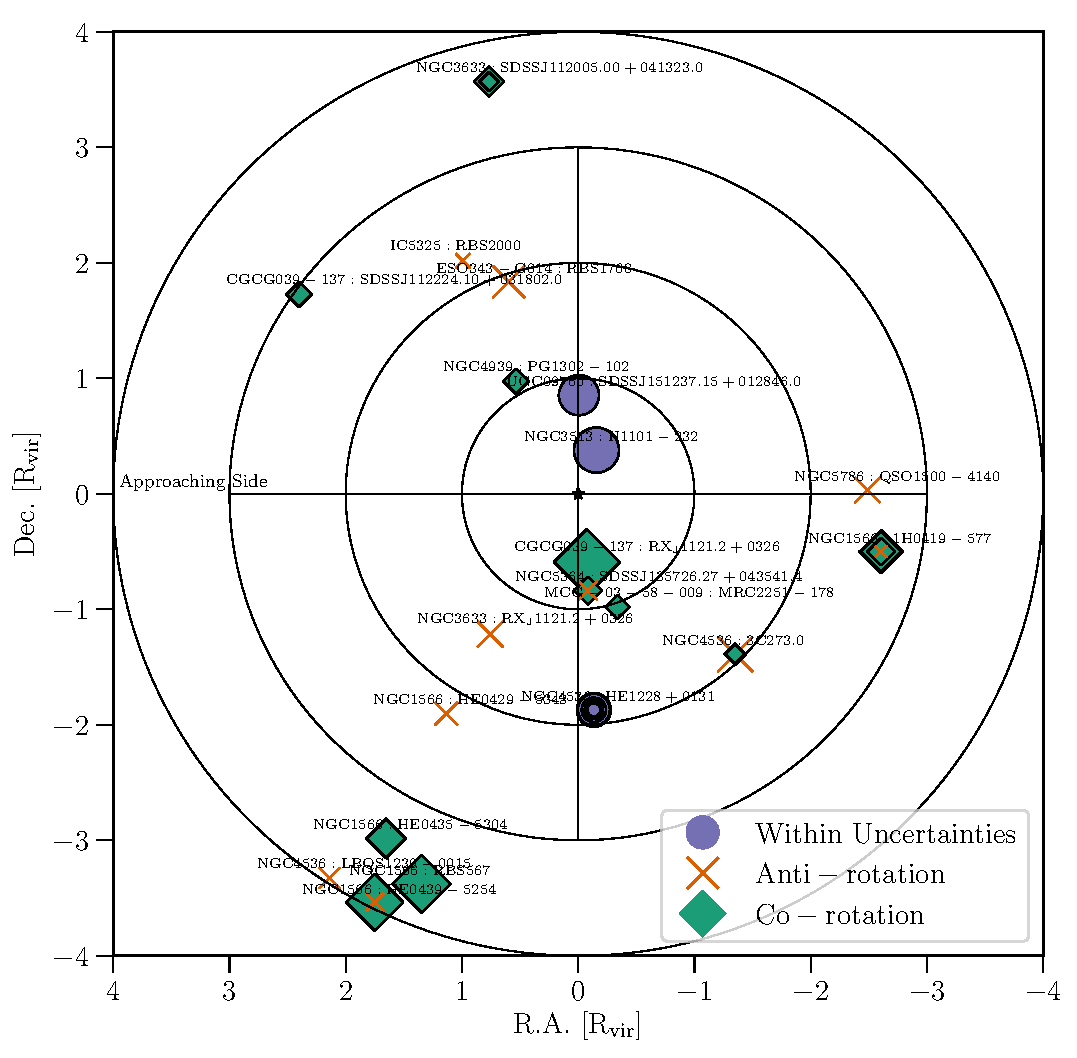
\includegraphics[width=0.90\textwidth]{SALT_map6.pdf}
        \caption{\small{A map of the locations of each absorber normalized with respect to the galaxy virial radius. Concentric rings indicate distances of 1, 2 and 3 $R_{vir}$. All galaxies are rotated to PA = 90, such that their major axis' are horizontal. The color and style of each point indicates the line-of-sight velocity compared to that of the rotation of the nearby galaxy. Green diamonds indicate co-rotation, red X's indicate anti-rotation, and purple circles indicate cases where either is possible due to a combination of orientation and velocity uncertainties. The size of each point is scaled to reflect the EW of the absorber. }}
%        \vspace{-5pt}
        \label{map}
\end{figure*}


%\begin{figure}[t!]
%\centering
%  \subfigure[]{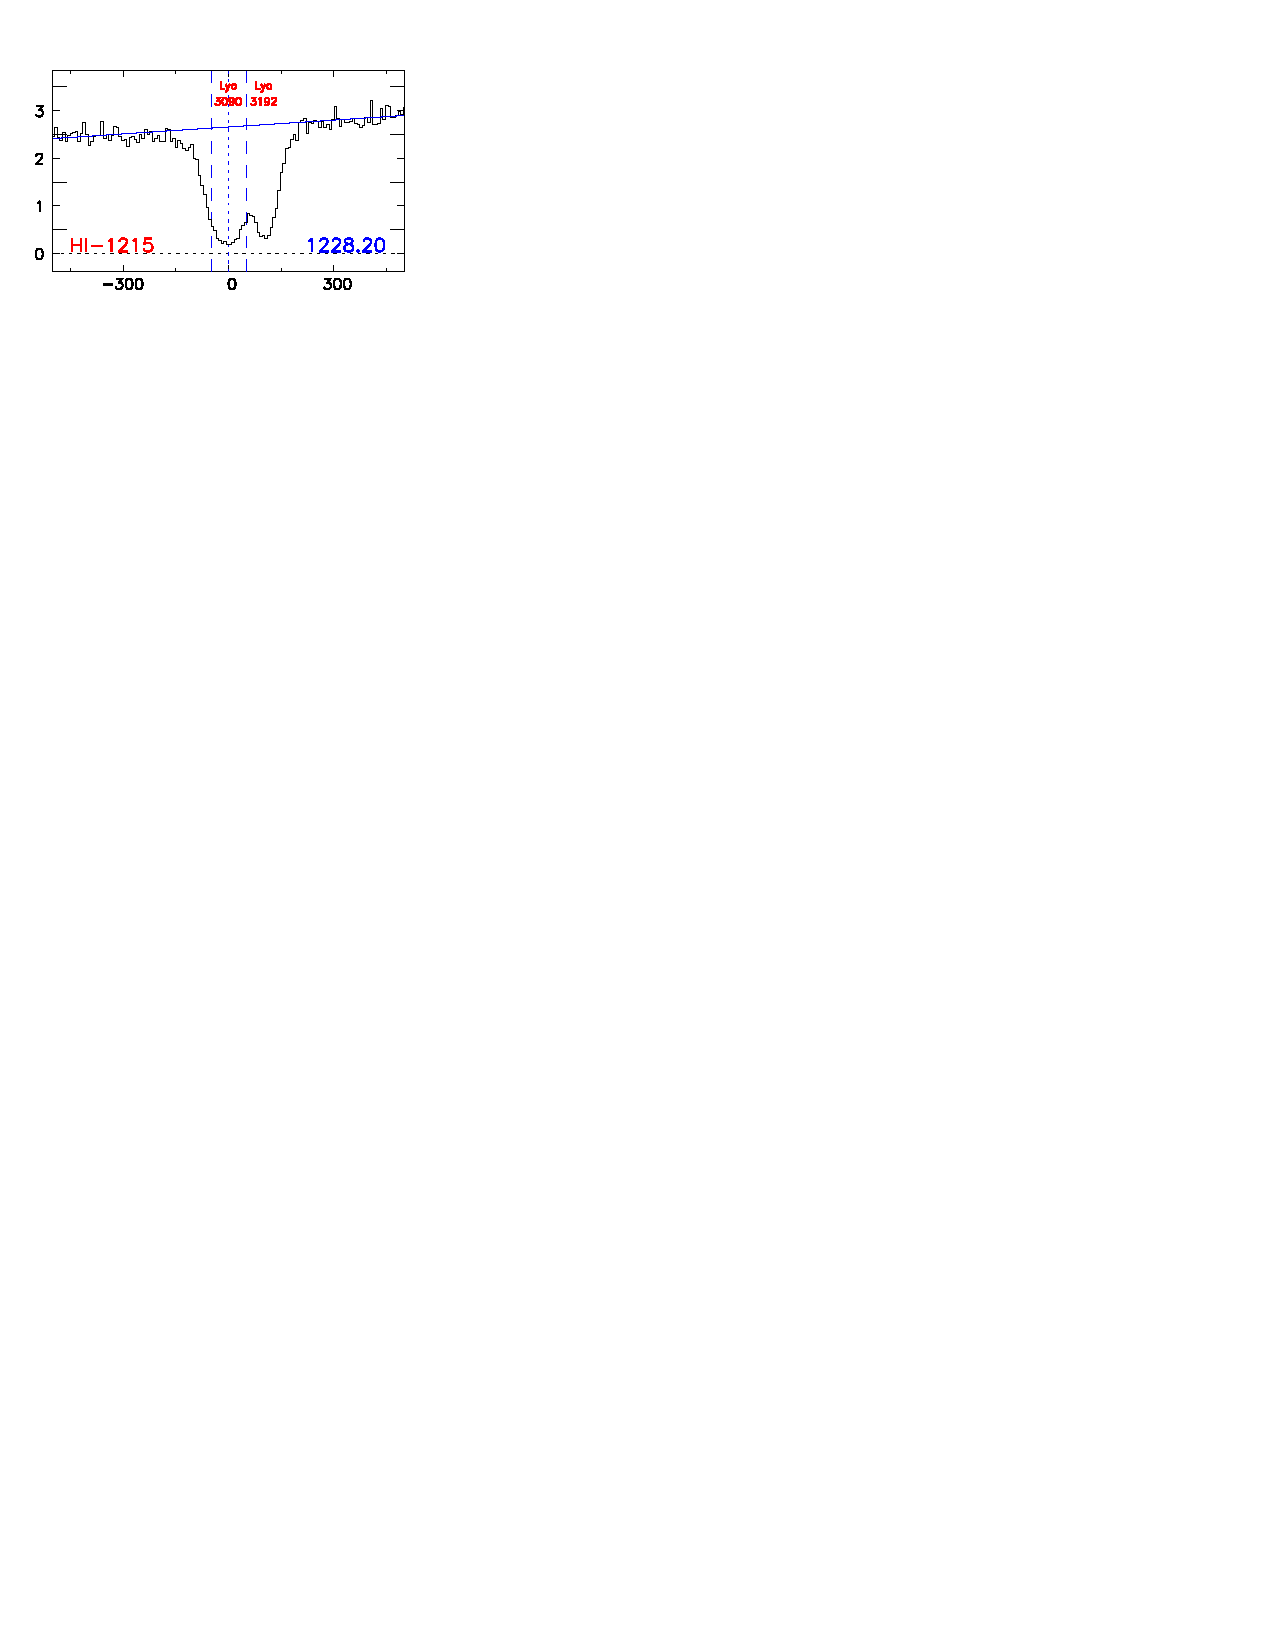
\includegraphics[width=0.87\linewidth]{fig2.pdf}}{\label{line}}
%  \subfigure[]{\includegraphics[width=1.\linewidth]{fig3.pdf}\label{impactmap}}
%  \caption{\small{a) An example of 2 Ly$\alpha$ lines found in the Mrk290 sightline at 3090 and 3192 . b) A map of \textit{all} galaxies within a 500 kpc impact parameter of target Mrk290 sightline and with velocity ($cz$) within 400 $\rm km\, s^{-1}$ of absorption detected at 3192 $\rm km\, s^{-1}$ (central black star). The galaxy NGC5987 ($v=3010$ $\rm km\, s^{-1}$, inclination = $65^{\circ}$) can be unambiguously paired with the Ly$\alpha$ absorption features at $v=3090, 3192$ $\rm km\, s^{-1}$ because it is the largest and closest galaxy in both physical and velocity space to the absorption feature.}}
%\vspace{5pt}
%\end{figure}




\section{Summary}



%\begin{table}[ht]\footnotesize
%\begin{center}
%\begin{tabular}{l l l}
% \hline \hline
% Statistic                				&  Blueshifted Absorbers   &     Redshifted Absorbers     \\ 
%  \hline \hline
% Number 	          			 		&     	22				&	26			\\
% Mean $EW$    \scriptsize $\rm [m\AA]$    &	$329 \pm 52$ 		&	$245 \pm 34$  	\\
%  
%\hline
%\end{tabular}
%\end{center}
%  \caption{\small{Average properties of the associated galaxy sample split into red and blue-shifted bins based on $\Delta v$.}}
%  \label{resultsTable}
%\end{table}


\vspace{10pt}


\acknowledgements

This research has made use of the NASA/IPAC Extragalactic Database (NED) which is operated by the Jet Propulsion Laboratory, California Institute of Technology, under contract with the National Aeronautics and Space Administration. Based on observations with the NASA/ESA \textit{Hubble Space Telescope}, obtained at the Space Telescope Science Institute (STScI), which is operated by the Association of Universities for Research in Astronomy, Inc., under NASA contract NAS 5-26555. \textbf{SALT ACKNOWLEDGEMENT}. Spectra were retrieved from the Barbara A. Mikulski Archive for Space Telescopes (MAST) at STScI. Over the course of this study, D.M.F. and B.P.W. were supported by grant AST-1108913, awarded by the US National Science Foundation, and by NASA grants \textit{HST}-AR-12842.01-A, \textit{HST}-AR-13893.01-A, and \textit{HST}-GO-14240 (STScI). 

\facility{HST (COS)}

\appendix

\section{Rotation Curves}
Here we present rotation curves with finder charts indicating the slit position for each galaxy observed with SALT. 

\begin{figure}[t!]
\centering
  \subfigure[]{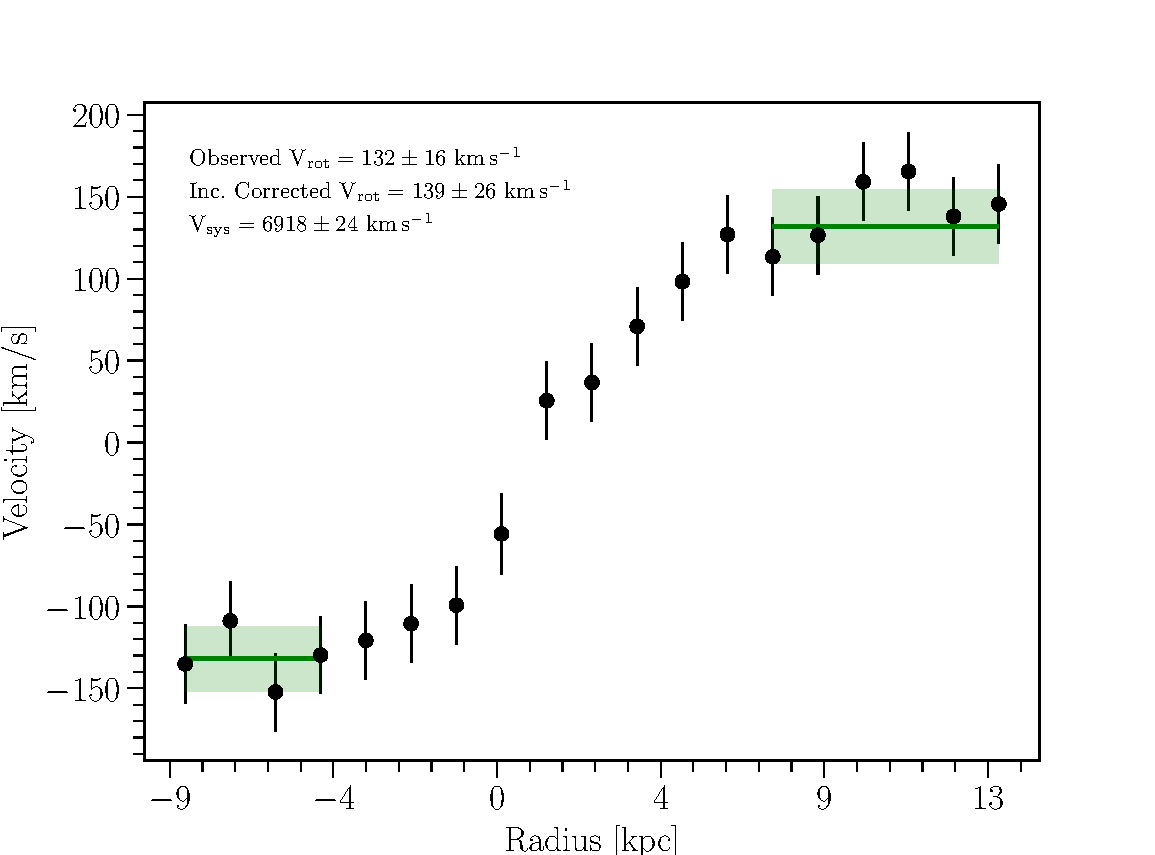
\includegraphics[width=.54\linewidth]{CGCG039-137_2_rotation_curve_xphys_helio_vobs_vrotObs_new4.pdf}}{\label{rotationcurve_CGCG039-137}}
  \subfigure[]{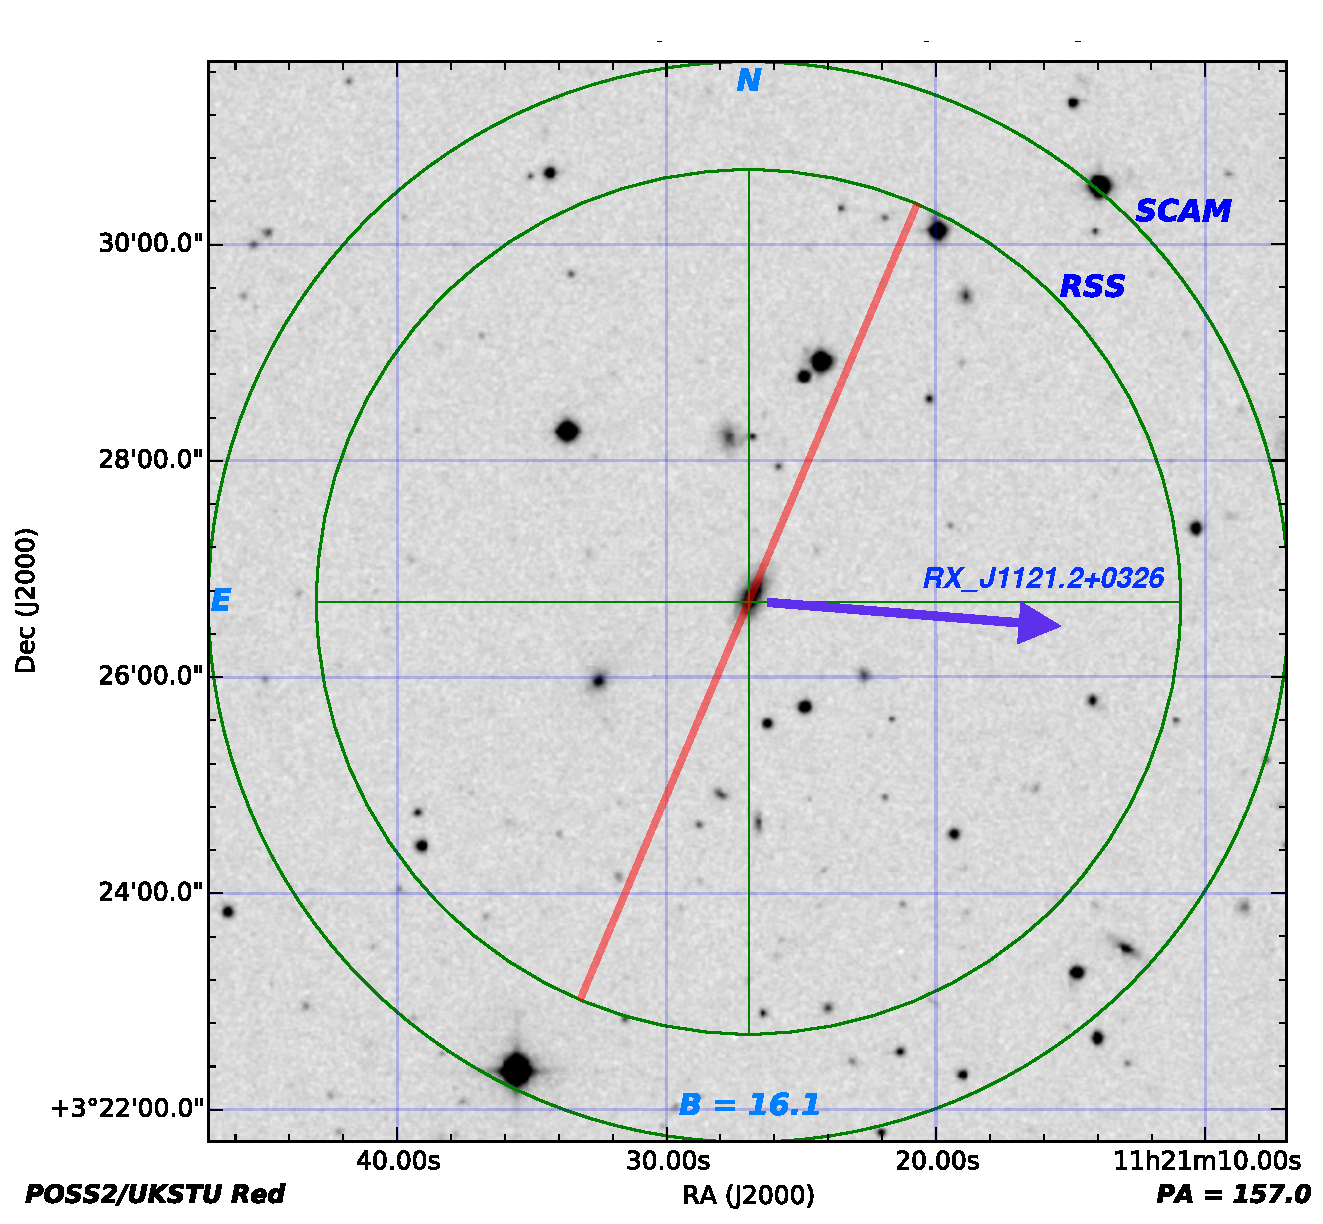
\includegraphics[width=0.45\linewidth]{CGCG039-137_Finding_chart.pdf}\label{finderchart_CGCG039-137}}
  \caption{\small{a) Rotation curve of CGCG039-137. The solid green line indicates the weighted mean velocity over the corresponding x-axis region, and the shaded green indicates the 1$\sigma$ error in the mean. b) SALT finder chart for CGCG039-137 showing the position of the slit in red.}}
\vspace{5pt}
\end{figure}


\begin{figure}[t!]
\centering
  \subfigure[]{\includegraphics[width=.54\linewidth]{IC5325_2_rotation_curve_xphys_helio_vobs_vrotObs_new4.pdf}}{\label{rotationcurve_IC5325}}
  \subfigure[]{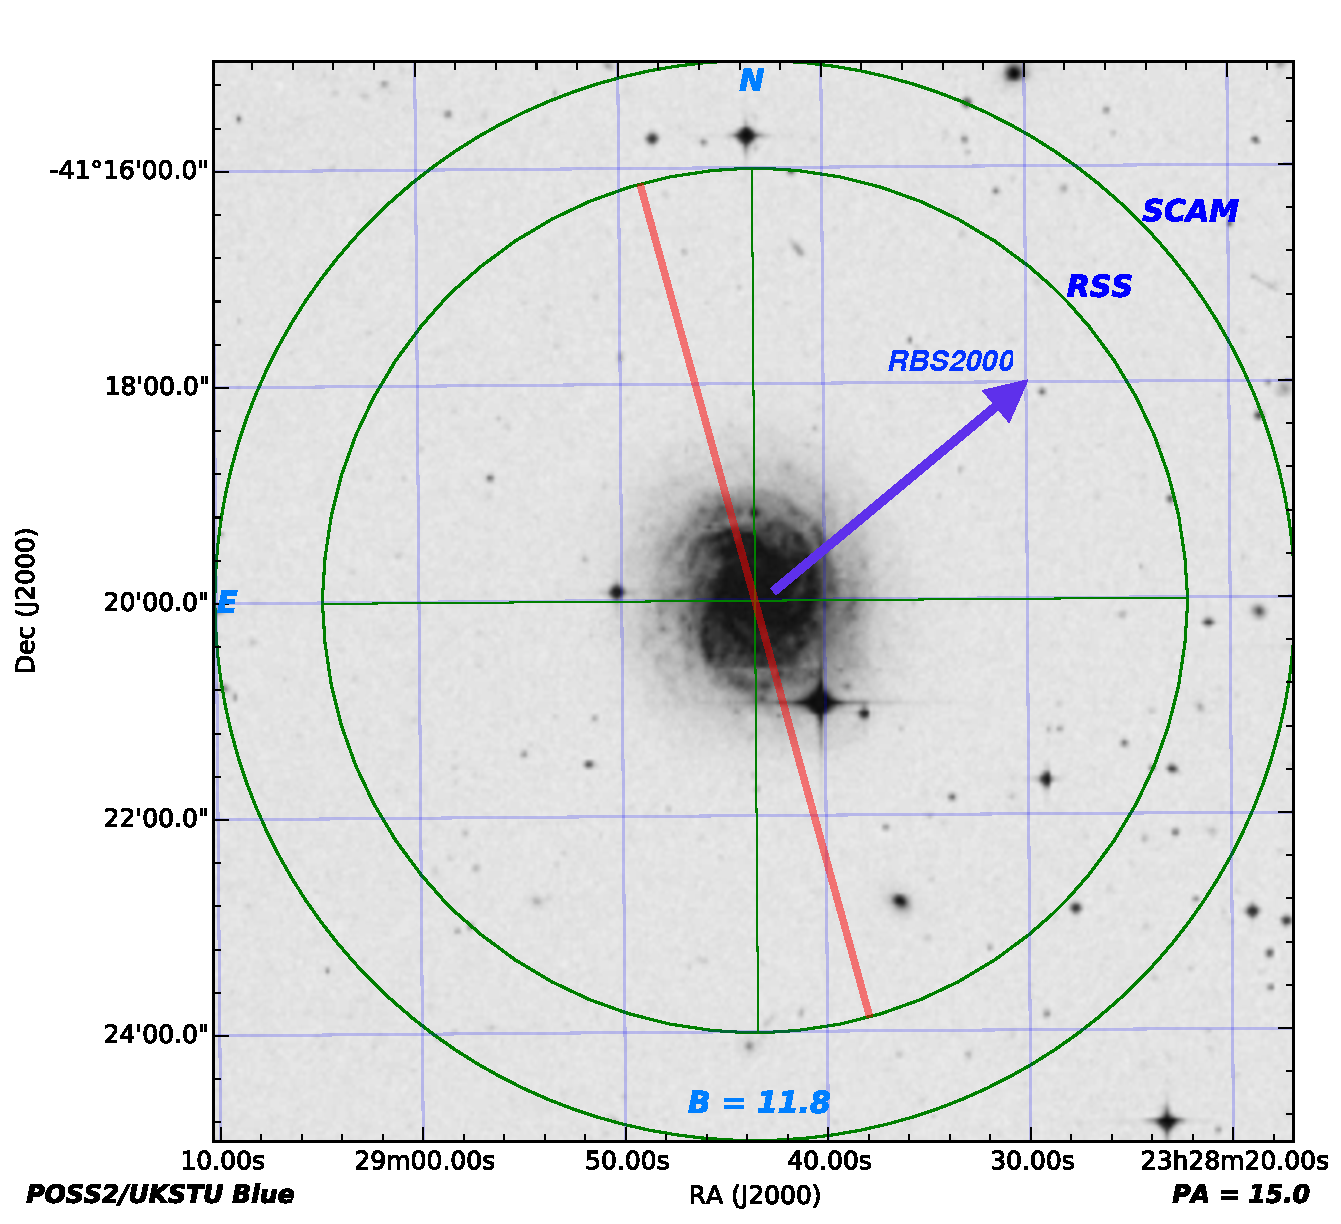
\includegraphics[width=0.45\linewidth]{IC5325_FindingChart.pdf}\label{finderchart_IC5325}}
  \caption{\small{a) Rotation curve of IC5325. The solid green line indicates the weighted mean velocity over the corresponding x-axis region, and the shaded green indicates the 1$\sigma$ error in the mean. b) SALT finder chart for IC5325 showing the position of the slit in red.}}
\vspace{5pt}
\end{figure}


\begin{figure}[t!]
\centering
  \subfigure[]{\includegraphics[width=.54\linewidth]{MCG-03-58-009_2_rotation_curve_xphys_helio_vobs_vrotObs_new4.pdf}}{\label{rotationcurve_MCG-03-58-009}}
  \subfigure[]{\includegraphics[width=0.45\linewidth]{MCG-03-58-009_FindingChart.pdf}\label{finderchart_MCG-03-58-009}}
  \caption{\small{a) Rotation curve of MCG-03-58-009. The solid green line indicates the weighted mean velocity over the corresponding x-axis region, and the shaded green indicates the 1$\sigma$ error in the mean. b) SALT finder chart for MCG-03-58-009 showing the position of the slit in red.}}
\vspace{5pt}
\end{figure}


\begin{figure}[t!]
\centering
  \subfigure[]{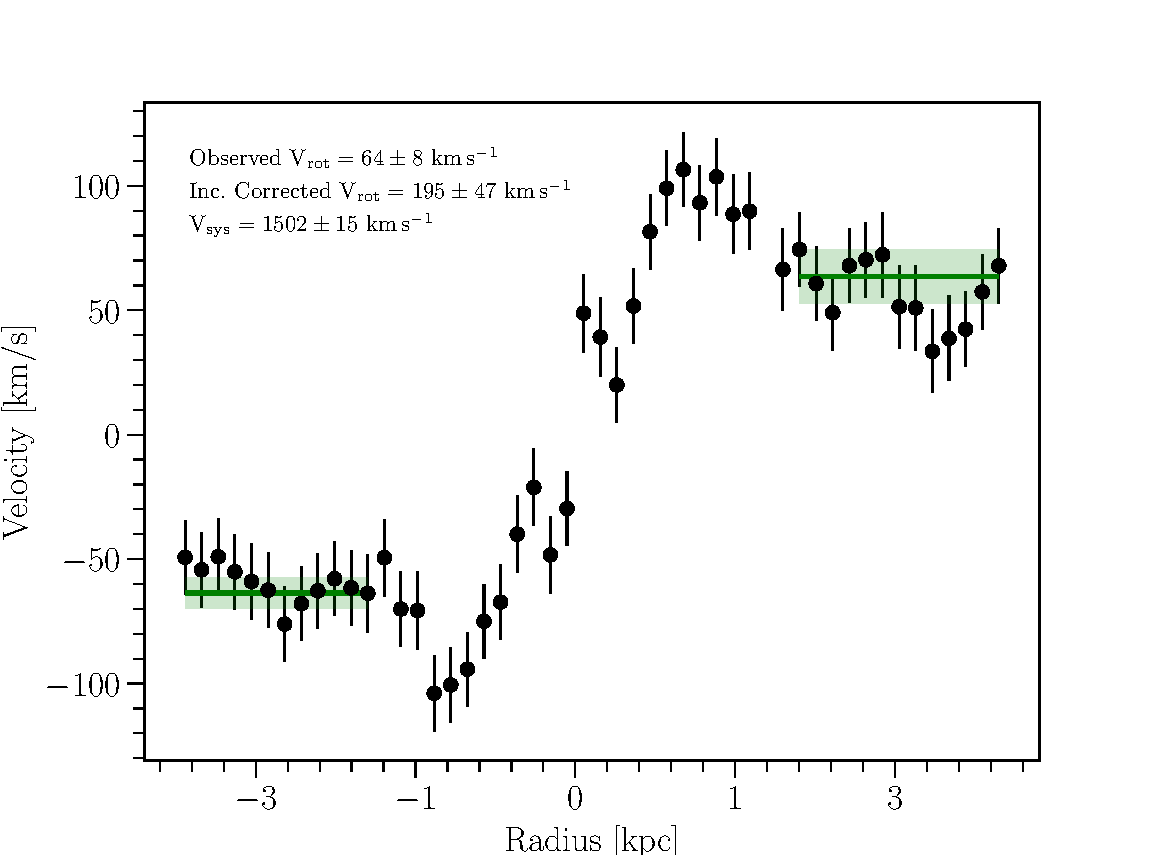
\includegraphics[width=.54\linewidth]{NGC1566_2_rotation_curve_xphys_helio_vobs_vrotObs_new4.pdf}}{\label{rotationcurve_NGC1566}}
  \subfigure[]{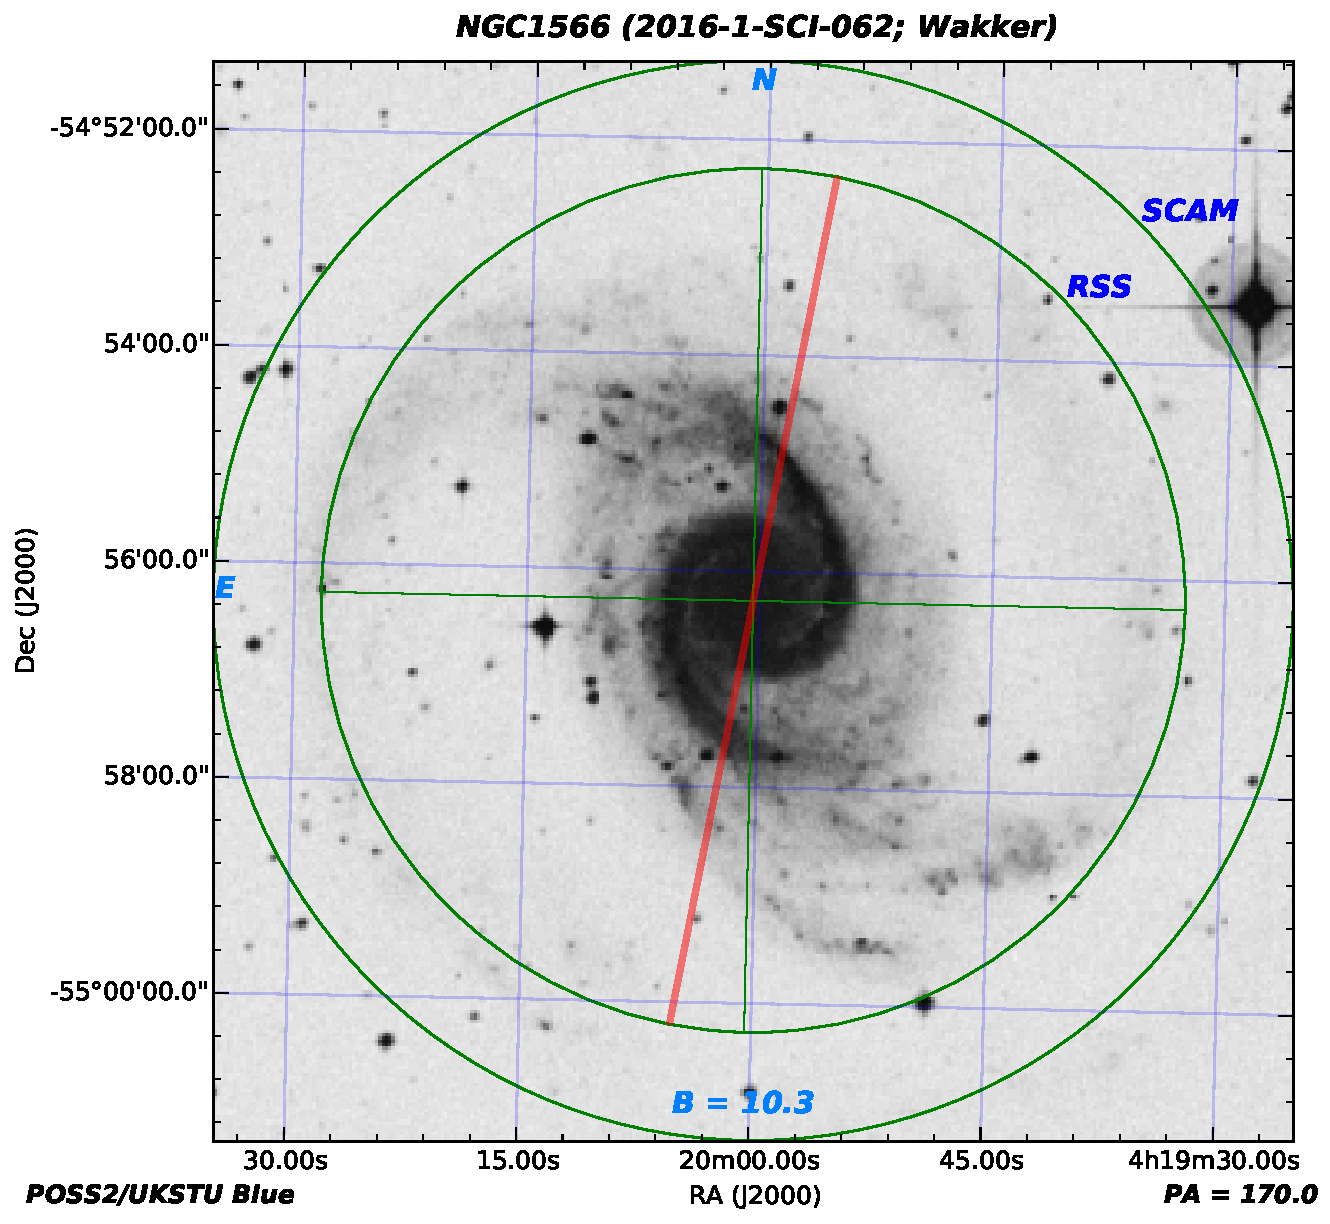
\includegraphics[width=0.45\linewidth]{NGC1566_FindingChart.pdf}\label{finderchart_NGC1566}}
  \caption{\small{a) Rotation curve of NGC1566. The solid green line indicates the weighted mean velocity over the corresponding x-axis region, and the shaded green indicates the 1$\sigma$ error in the mean. b) SALT finder chart for NGC1566 showing the position of the slit in red.}}
\vspace{5pt}
\end{figure}


\begin{figure}[t!]
\centering
  \subfigure[]{\includegraphics[width=.54\linewidth]{NGC3513_2_rotation_curve_xphys_helio_vobs_vrotObs_new4.pdf}}{\label{rotationcurve_NGC3513}}
  \subfigure[]{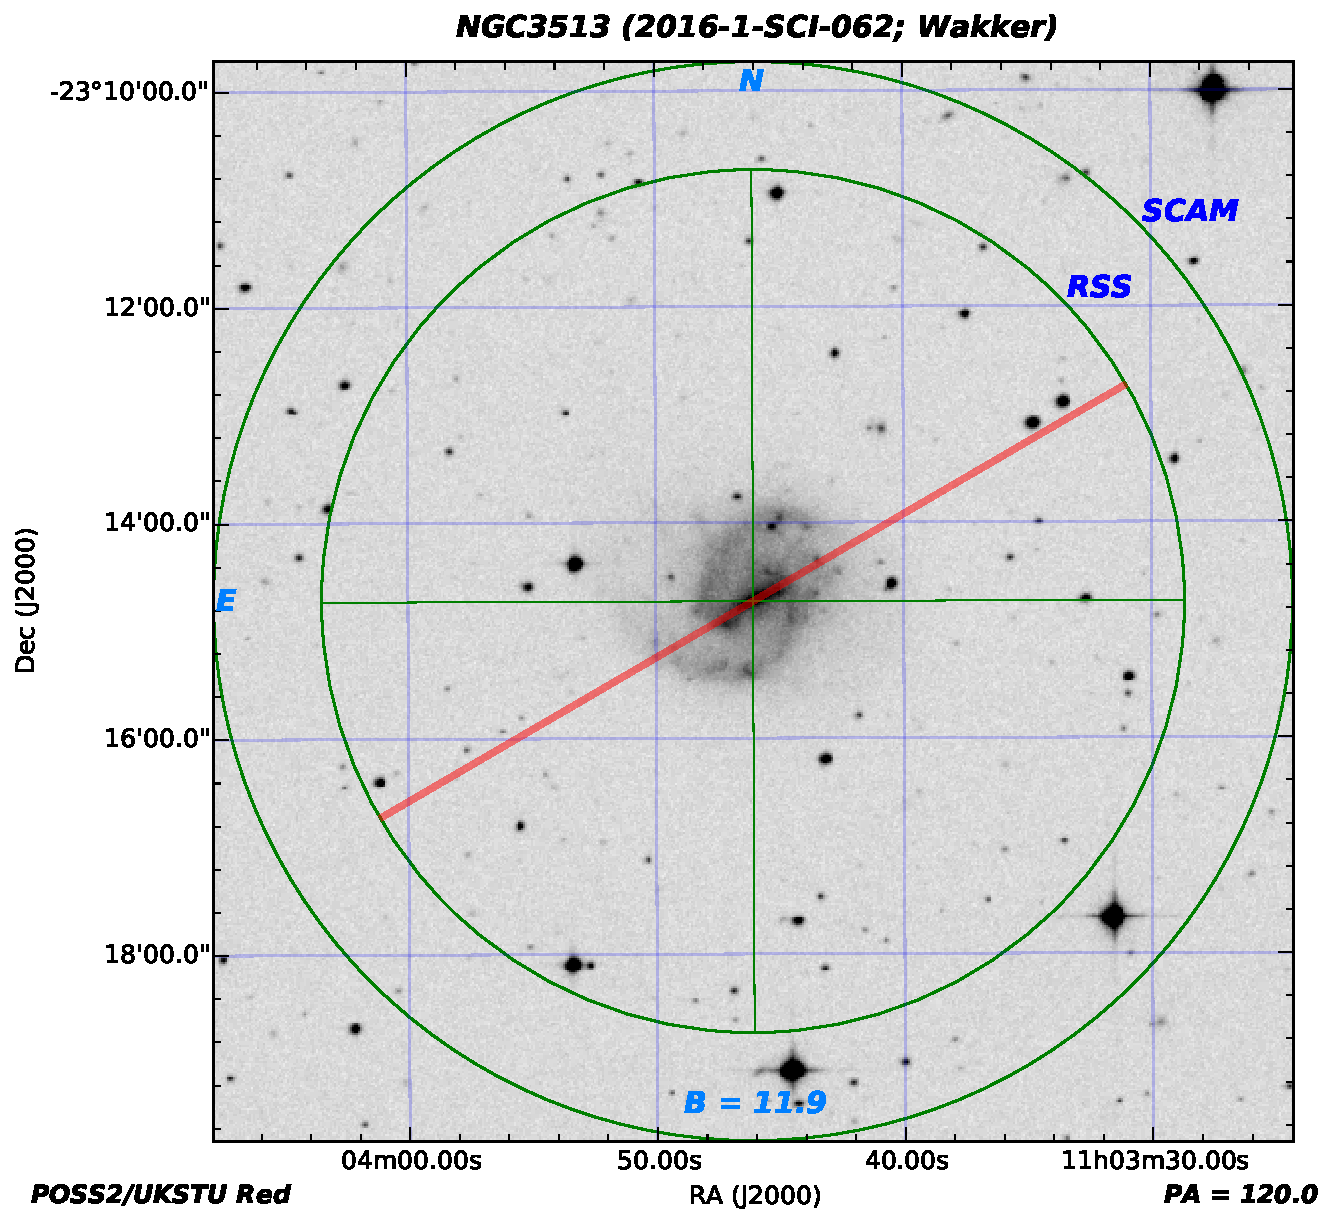
\includegraphics[width=0.45\linewidth]{NGC3513_Finding_chart.pdf}\label{finderchart_NGC3513}}
  \caption{\small{a) Rotation curve of NGC3513. The solid green line indicates the weighted mean velocity over the corresponding x-axis region, and the shaded green indicates the 1$\sigma$ error in the mean. b) SALT finder chart for NGC3513 showing the position of the slit in red.}}
\vspace{5pt}
\end{figure}


\begin{figure}[t!]
\centering
  \subfigure[]{\includegraphics[width=.54\linewidth]{NGC3633_2_rotation_curve_xphys_helio_vobs_vrotObs_new4.pdf}}{\label{rotationcurve_NGC3633}}
  \subfigure[]{\includegraphics[width=0.45\linewidth]{NGC3633_FindingChart.pdf}\label{finderchart_NGC3633}}
  \caption{\small{a) Rotation curve of NGC4536. The solid green line indicates the weighted mean velocity over the corresponding x-axis region, and the shaded green indicates the 1$\sigma$ error in the mean. b) SALT finder chart for NGC3633 showing the position of the slit in red.}}
\vspace{5pt}
\end{figure}


\begin{figure}[t!]
\centering
  \subfigure[]{\includegraphics[width=.54\linewidth]{NGC4536_2_rotation_curve_xphys_helio_vobs_vrotObs_new4.pdf}}{\label{rotationcurve_NGC4536}}
  \subfigure[]{\includegraphics[width=0.45\linewidth]{NGC4536_FindingChart.pdf}\label{finderchart_NGC4536}}
  \caption{\small{a) Rotation curve of NGC4536. The solid green line indicates the weighted mean velocity over the corresponding x-axis region, and the shaded green indicates the 1$\sigma$ error in the mean. b) SALT finder chart for NGC4536 showing the position of the slit in red.}}
\vspace{5pt}
\end{figure}


\begin{figure}[t!]
\centering
  \subfigure[]{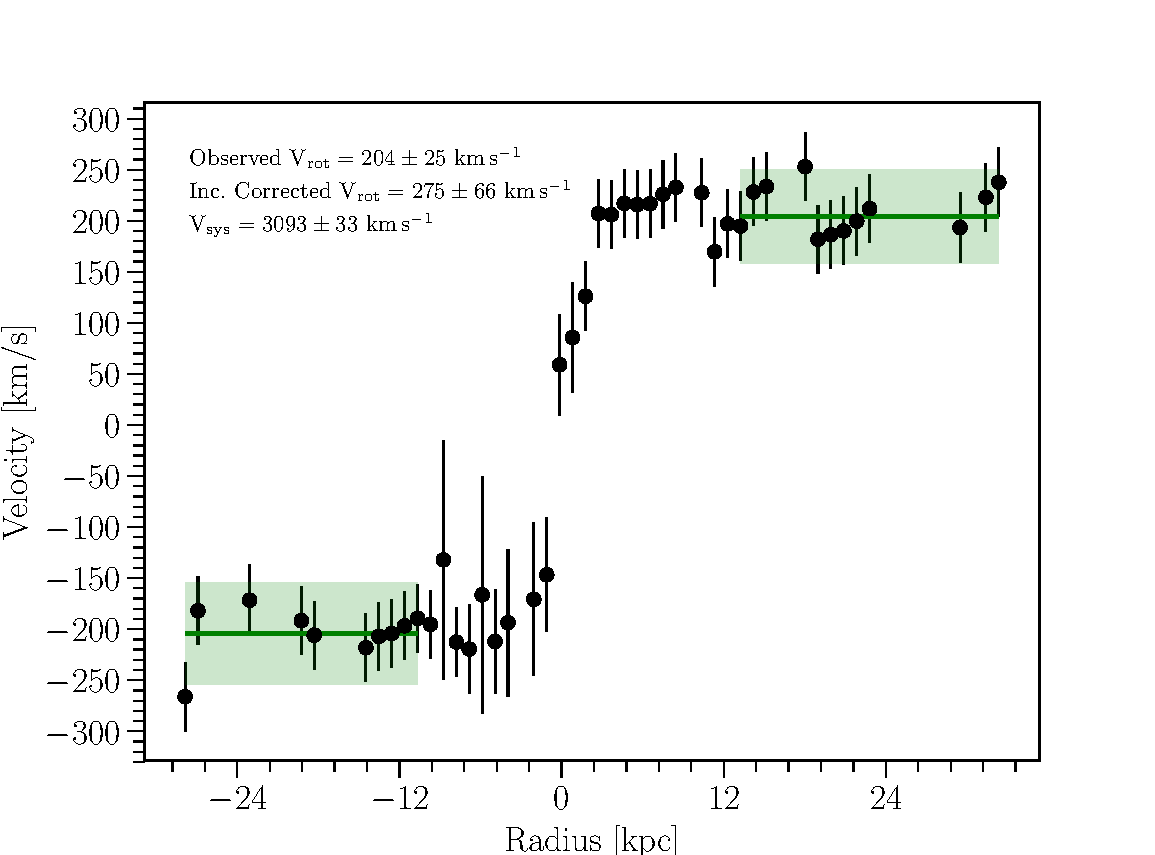
\includegraphics[width=.54\linewidth]{NGC4939_2_rotation_curve_xphys_helio_vobs_vrotObs_new4.pdf}}{\label{rotationcurve_NGC4939}}
  \subfigure[]{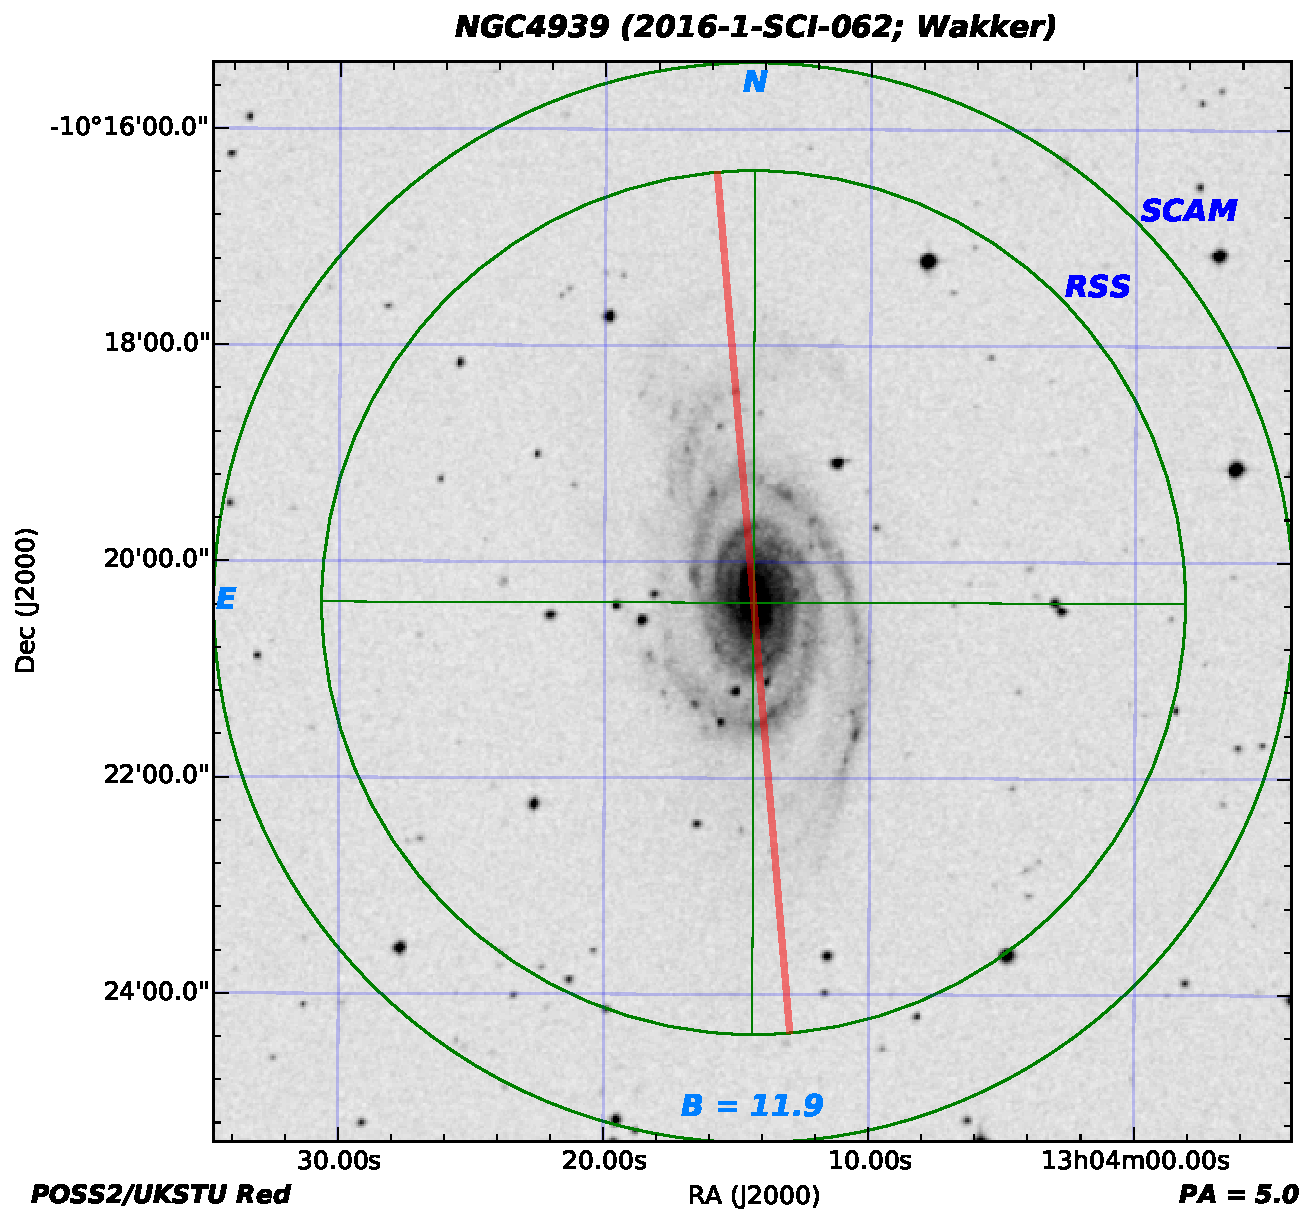
\includegraphics[width=0.45\linewidth]{NGC4939_FindingChart.pdf}\label{finderchart_NGC4939}}
  \caption{\small{a) Rotation curve of NGC4939. The solid green line indicates the weighted mean velocity over the corresponding x-axis region, and the shaded green indicates the 1$\sigma$ error in the mean. b) SALT finder chart for NGC4939 showing the position of the slit in red.}}
\vspace{5pt}
\end{figure}


\begin{figure}[t!]
\centering
  \subfigure[]{\includegraphics[width=.54\linewidth]{NGC5364_2_rotation_curve_xphys_helio_vobs_vrotObs_new4.pdf}}{\label{rotationcurve_NGC5364}}
  \subfigure[]{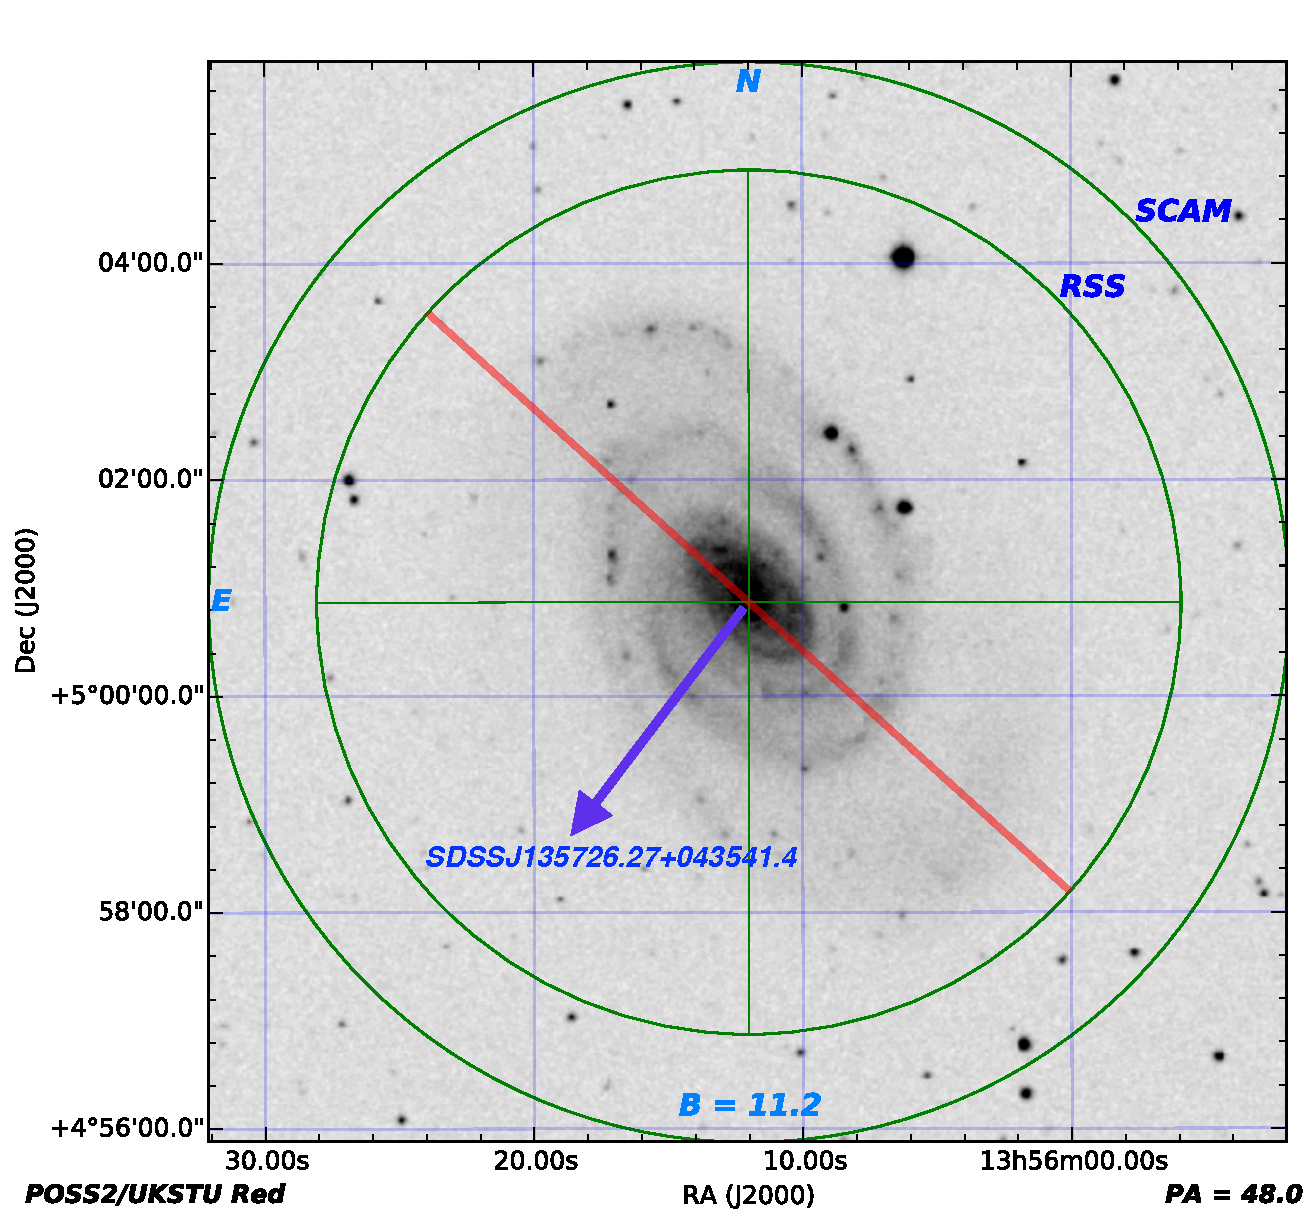
\includegraphics[width=0.45\linewidth]{NGC5364_FindingChart.pdf}\label{finderchart_NGC5364}}
  \caption{\small{a) Rotation curve of NGC5364. The solid green line indicates the weighted mean velocity over the corresponding x-axis region, and the shaded green indicates the 1$\sigma$ error in the mean. b) SALT finder chart for NGC5364 showing the position of the slit in red.}}
\vspace{5pt}
\end{figure}


\begin{figure}[t!]
\centering
  \subfigure[]{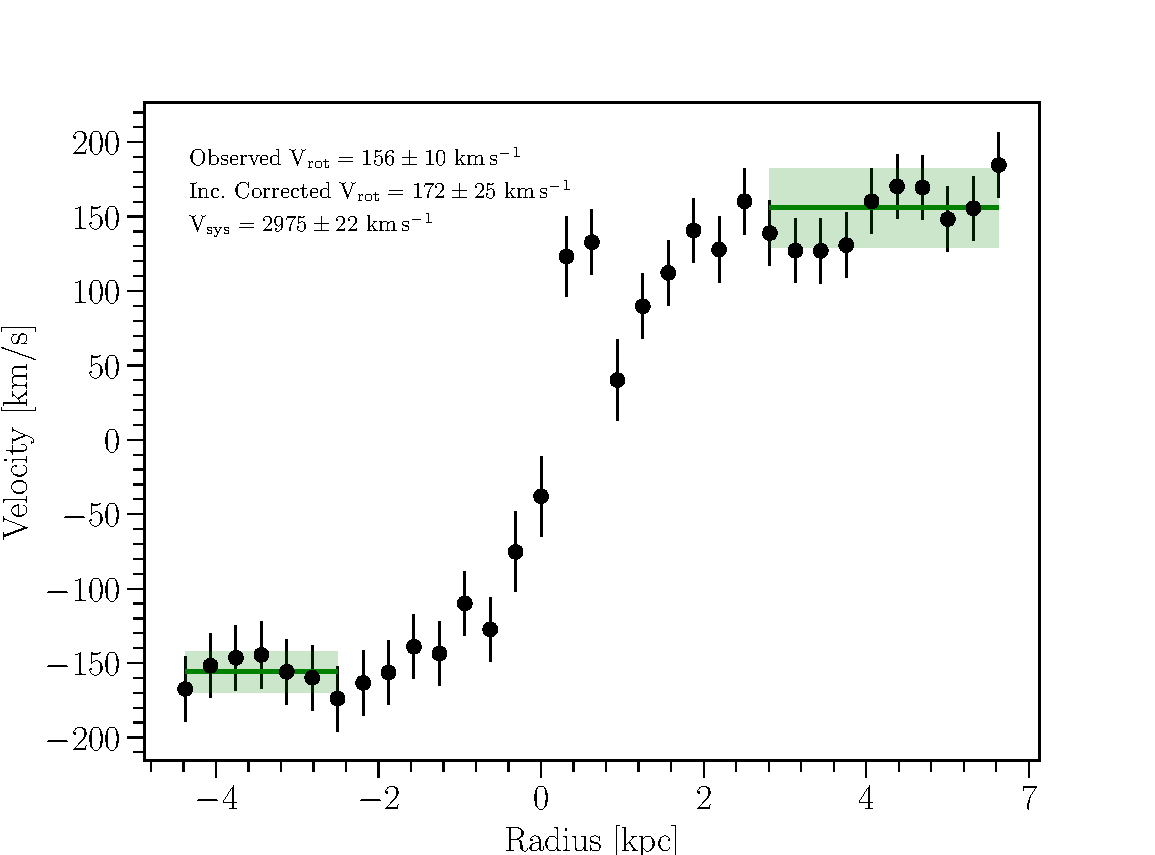
\includegraphics[width=.54\linewidth]{NGC5786_2_rotation_curve_xphys_helio_vobs_vrotObs_new4.pdf}}{\label{rotationcurve_NGC5786}}
  \subfigure[]{\includegraphics[width=0.45\linewidth]{NGC5786_FindingChart.pdf}\label{finderchart_NGC5786}}
  \caption{\small{a) Rotation curve of NGC5786. The solid green line indicates the weighted mean velocity over the corresponding x-axis region, and the shaded green indicates the 1$\sigma$ error in the mean. b) SALT finder chart for NGC5786 showing the position of the slit in red.}}
\vspace{5pt}
\end{figure}


\begin{figure}[t!]
\centering
  \subfigure[]{\includegraphics[width=.54\linewidth]{RFGC3781_2_rotation_curve_xphys_helio_vobs_vrotObs_new4.pdf}}{\label{rotationcurve_RFGC3781}}
  \subfigure[]{\includegraphics[width=0.45\linewidth]{RFGC3781_FindingChart.pdf}\label{finderchart_RFGC3781}}
  \caption{\small{a) Rotation curve of NGC5364. The solid green line indicates the weighted mean velocity over the corresponding x-axis region, and the shaded green indicates the 1$\sigma$ error in the mean. b) SALT finder chart for NGC5364 showing the position of the slit in red.}}
\vspace{5pt}
\end{figure}



%\nocite{*}
%\bibliography{rotation_bib}
\bibliography{/Users/frenchd/Research/bib}{}
\bibliographystyle{apj}

\end{document}
